\documentclass[10pt]{article}		% sets document class
\usepackage{tgpagella}
\usepackage{tgheros}
\usepackage[usenames,dvipsnames]{pstricks}
\usepackage{epsfig}
\usepackage{pst-grad} 				% enables gradients
\usepackage{pst-plot} 				% enables axes
\usepackage[space]{grffile} 		% enables spaces in paths
\usepackage{etoolbox} 				% enables spaces in paths
\makeatletter 						% enables spaces in paths
\patchcmd\Gread@eps{\@inputcheck#1 }{\@inputcheck"#1"\relax}{}{}
\makeatother
\usepackage[margin=1.0in]{geometry}	% sets paper size
\usepackage{amssymb}				% enables formulas
\usepackage{amsmath}				% enables formulas
\usepackage[utf8]{inputenc}			% enables diacritical input
\usepackage{graphicx}				% enables graphics
\graphicspath{ {images/} }			% sets graphics path
\usepackage{chngcntr}				% enables counter
\counterwithin{table}{subsection}	% enables table pre-labels
\counterwithin{figure}{subsection}	% enables figure pre-labels
\usepackage[labelsep=endash, labelfont=bf]{caption}	% sets figure and caption separator
%\usepackage{indentfirst}			% enables indent on first paragraphs
\linespread{1.1}					% sets spacing to 1.5
\setlength{\parskip}{0.5em}			% sets paragraph spacing to 1m
\usepackage{gensymb}				% enables symbols
\usepackage{endnotes}				% enables endnotes
\usepackage{afterpage}				% enables afterpage capability
\setcounter{secnumdepth}{3}			% sets counter recognitions to sssection for label capability
\numberwithin{equation}{section}
\makeatletter						% set figure labels to center
\g@addto@macro\@floatboxreset\centering
\makeatother
\usepackage{setspace}				% enables environments for spacing
\usepackage{graphicx}				% allows table usage
\usepackage{hyperref}				% enables hyperlinks
\hypersetup{colorlinks=false, linkcolor=cyan, urlcolor=cyan, linktoc=page} % sets hyperlink colors
\usepackage{accents}				% enables accents
\usepackage{textcomp} 				% enables copyright
\usepackage{tabto}					% enables tabbing
\setlength\parindent{0pt}			% sets no indents
\usepackage[framed]{mcode} 			% enables code boxes
\usepackage{titlesec}				% enables title formatting
\titleformat{\part}{\filcenter\huge\bfseries}{}{}{}
\usepackage{float}
\newcommand{\pder}[2]{\frac{\partial#1}{\partial#2}}			% partial command
\newcommand{\psder}[2]{\dfrac{\partial^2#1}{\partial#2^2}}		% partial command
\newcommand{\ptder}[2]{\dfrac{\partial^3#1}{\partial#2^3}}		% partial command
\newcommand{\pfder}[2]{\dfrac{\partial^4#1}{\partial#2^4}}		% partial command
\newcommand{\pdx}{\frac{\partial}{\partial x}}					% partial command
\newcommand{\pdy}{\frac{\partial}{\partial y}}					% partial command
\newcommand{\pdz}{\frac{\partial}{\partial z}}					% partial command

\begin{document}

\newcommand{\stoptocwriting}{%
	\addtocontents{toc}{\protect\setcounter{tocdepth}{-5}}}
\newcommand{\resumetocwriting}{%
	\addtocontents{toc}{\protect\setcounter{tocdepth}{\arabic{tocdepth}}}}

\stoptocwriting
\part*{\underline{AERO 430 -- Numerical Simulation} \\ \Large Exact Solution of the Finite Difference Equations \\ \large Ross B. Alexander}
\resumetocwriting

\vfill

\begin{figure}[h]
	\begin{center}
	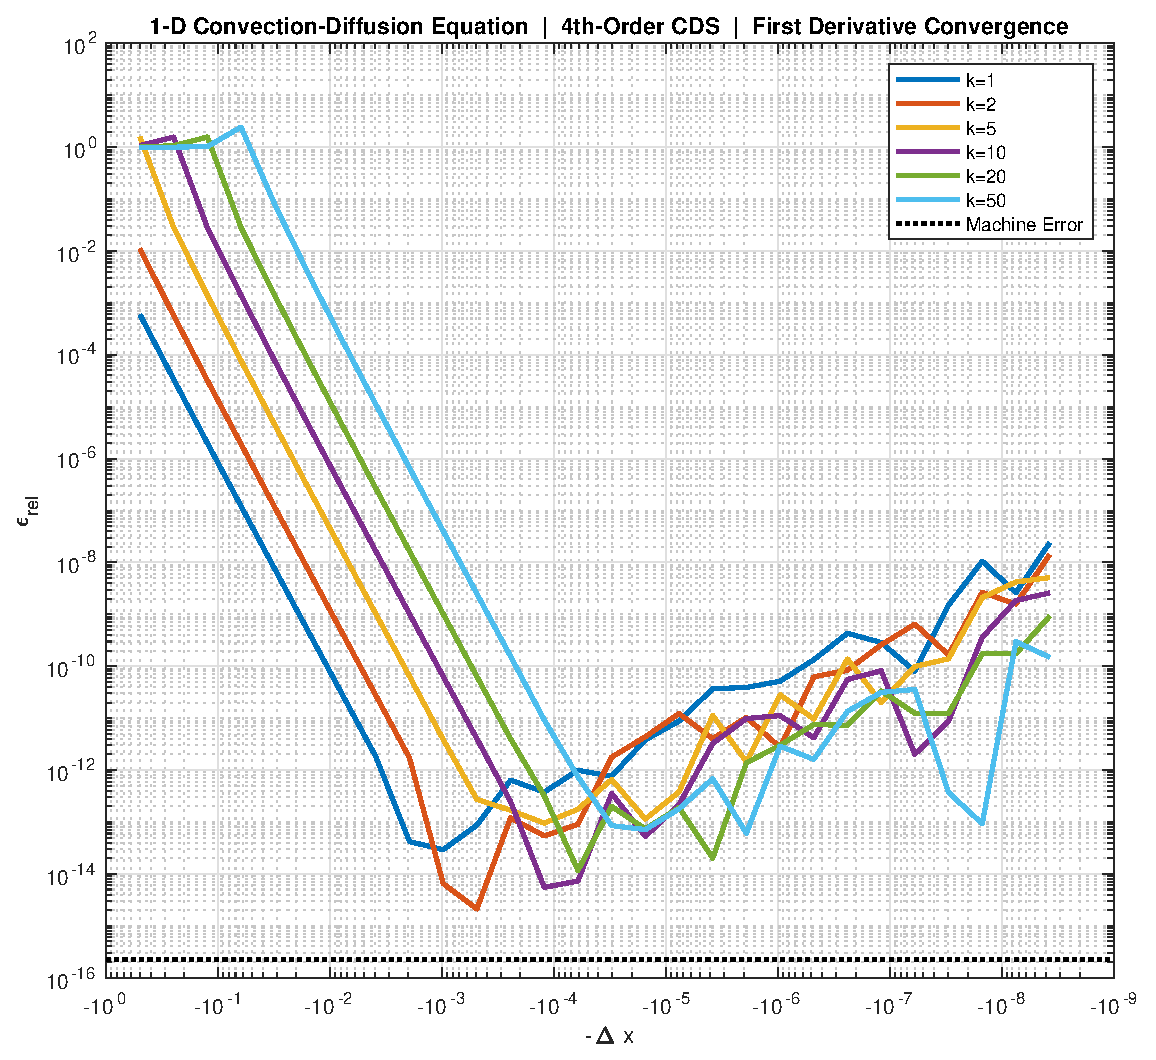
\includegraphics[width = 0.9\linewidth]{1dconv4oconv}
	\end{center}
\end{figure}

\vspace{80pt}

\newpage

\tableofcontents

\newpage

\section{Model Problems}

\subsection{1-D Diffusion Equation}

The \textit{first} model second-order linear ordinary differential equation boundary-value problem consists of:
\begin{itemize}
	\item the one-dimensional second-order linear ordinary differential equation:
	\begin{equation}
	-u''(x)+k^2u(x)=k^2x \qquad x \in [0, 1]
	\end{equation}
	\item the boundary conditions:
	\begin{equation}
	u(0) = 0 \quad \textnormal{and} \quad u(1) = 0 
	\end{equation}
\end{itemize}
The physical model of the second-order linear ordinary differential equation boundary-value problem is that of (1) the temperature of a bar for uniaxial heat conduction, and (2) the deflection of a beam for uniaxial deformation with distributed elastic restraint.


\subsection{1-D Harmonic Wave Equation}

The \textit{second} model second-order linear ordinary differential equation boundary-value problem consists of:
\begin{itemize}
	\item the one-dimensional second-order linear ordinary differential equation:
	\begin{equation}
	u''(x)+k^2u(x)=k^2x \qquad x \in [0, 1]
	\end{equation}
	\item the boundary conditions:
	\begin{equation}
	u(0) = 0 \quad \textnormal{and} \quad u(1) = 0 
	\end{equation}
\end{itemize}
The physical model of the second-order linear ordinary differential equation boundary-value problem is that of the amplitude of standing waves for uniaxial forced vibration of a bar.

\subsection{1-D Convection-Diffusion Equation}

The \textit{third} model second-order linear ordinary differential equation boundary-value problem consists of:
\begin{itemize}
	\item the one-dimensional second-order linear ordinary differential equation:
	\begin{equation}
	- u''(x)+cu'(x)=0 \qquad x \in [0, 1]
	\end{equation}
	\item the boundary conditions:
	\begin{equation}
	u(0) = 0 \quad \textnormal{and} \quad u(1) = 1 
	\end{equation}
\end{itemize}
The physical model of the second-order linear ordinary differential equation boundary-value problem is that of the concentration of a flow property that convects and diffuses proportional to the constant $c$. For example, the convection-diffusion equation could represent the concentration of ink as a function of distance in a quasi-one-dimensional flow.

\subsection{2-D Orthotropic Diffusion Equation}

The \textit{fourth} model second-order linear ordinary differential equation boundary-value problem consists of:
\begin{itemize}
	\item the two-dimensional second-order linear partial differential equation:
	\begin{equation}
	\nabla \cdot (\mathbf{D} \nabla u) = 0 \qquad x,y \in [0, 1] \times [0, 1]
	\end{equation}
	\item the orthotropic diffusivity tensor:
	\begin{equation}
	\mathbf{D} = \begin{bmatrix}
	k^2 & 0 & 0 \\
	0 & 1 & 0 \\
	0 & 0 & 0
	\end{bmatrix}
	\end{equation}
	\item the simplified two-dimensional second-order linear partial differential equation:
	\begin{equation}
	k^2\psder{u}{x} + \psder{u}{y} = 0 \qquad x,y \in [0, 1] \times [0, 1]
	\end{equation}
	\item the boundary conditions:
	\begin{equation}
	\begin{split}
	u(x, 0) = 0 \qquad \qquad u(0, y) = 0  \\
	u(x, 1) = \sin{\pi x} \qquad u(1, y) = 0
	\end{split}
	\end{equation}
\end{itemize}

The physical model of the orthotropic diffusion equation is that of (1) electrical conduction through a medium that has orthotropic electrical conductivity, (2) magnetism of a material that has orthotropic magnetic permeability, (3) thermal conduction through a material that has orthotropic thermal conductivity, or (4) diffusion through a fluid that has orthotropic diffusivity.

\newpage

\section{Analytical Solutions}

\subsection{1-D Diffusion Equation}

Previously, it was shown that for the one-dimensional second-order linear ordinary differential equation with specified boundary conditions (reproduced below) that $u(x)$ is a solution to the differential equation on $x \in [0, 1]$.
\begin{equation}
-u''(x)+k^2u(x)=k^2x \qquad x \in [0, 1]
\end{equation}
\begin{equation}
u(0) = 0 \quad \textnormal{and} \quad u(1) = 0 
\end{equation}
\begin{equation}
u(x) = x - \frac{\sinh(kx)}{\sinh(k)}
\end{equation}

A plot of the analytical solution for values of $k$ is depicted in Figure \ref{fig:analytical_diff}:
\begin{figure}[H]
	\begin{center}
		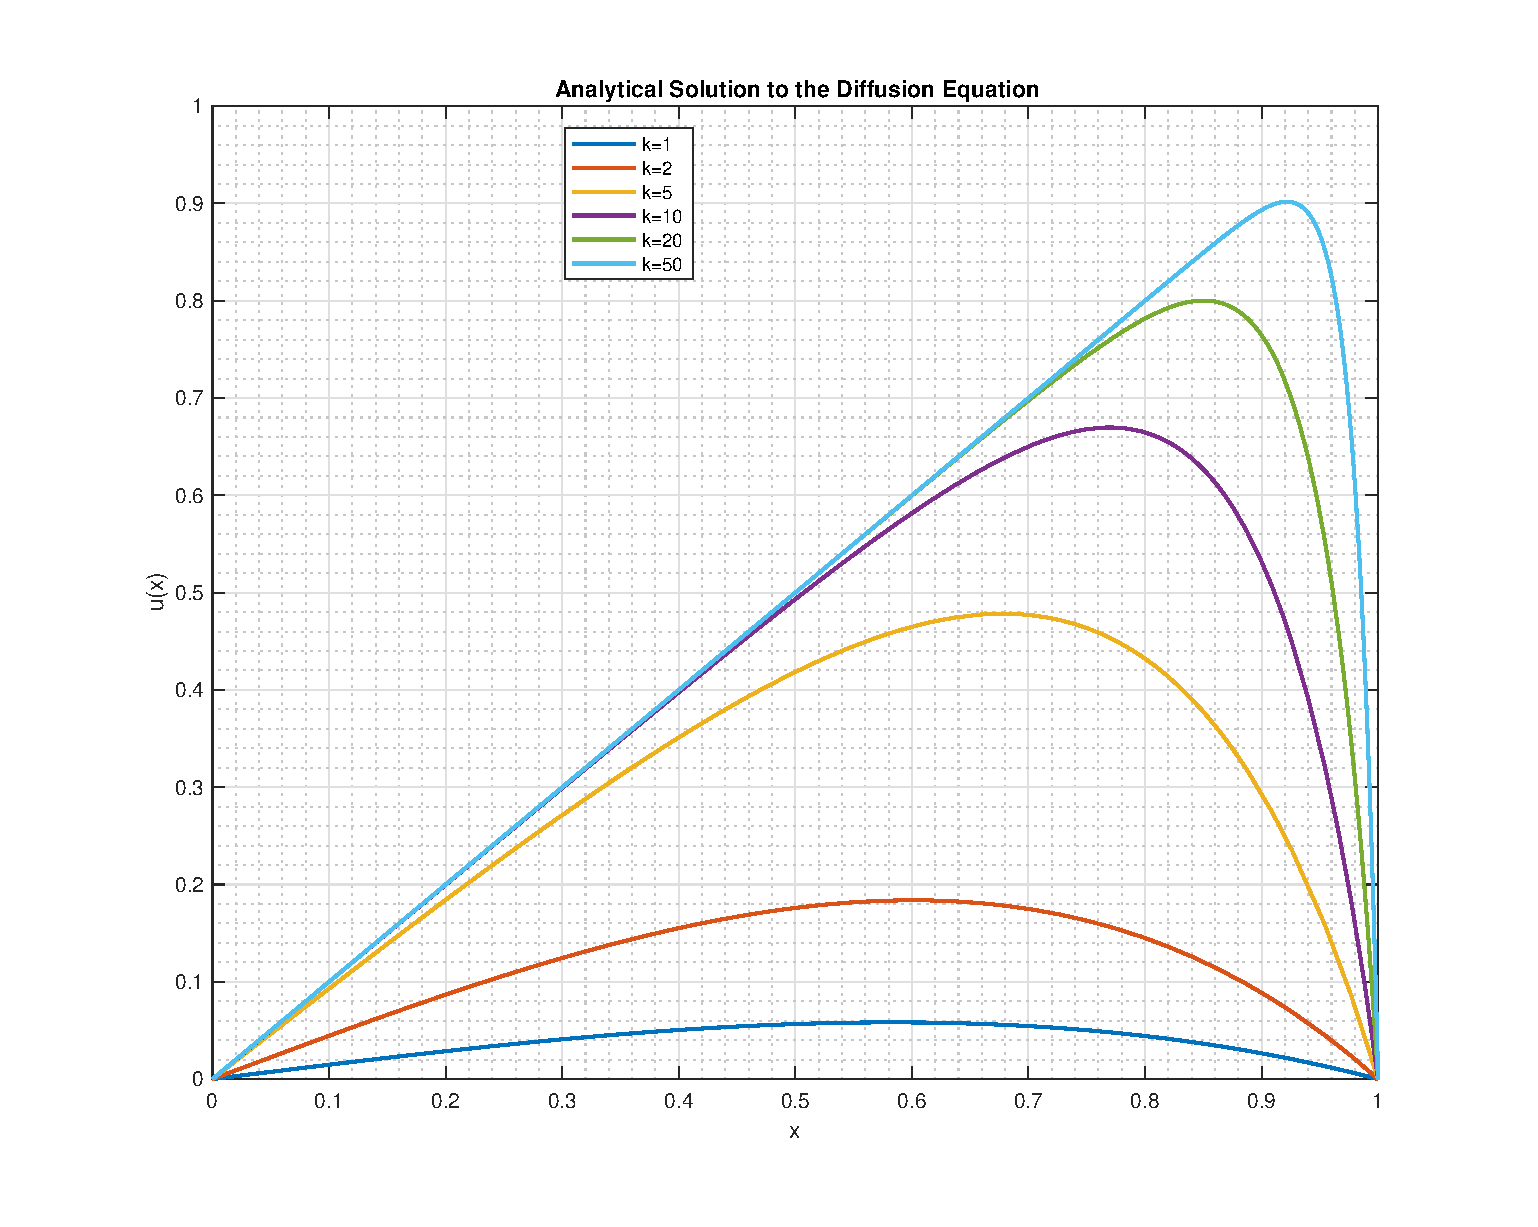
\includegraphics[width = 0.95\linewidth]{analytical_solution_diffusion}
		\caption{Analytical Solution to the Diffusion Equation for Values of $k$}
		\label{fig:analytical_diff}
	\end{center}
\end{figure}

\newpage

\subsection{1-D Harmonic Wave Equation}

Previously, it was shown that for the one-dimensional second-order linear ordinary differential equation with specified boundary conditions (reproduced below) that $u(x)$ is a solution to the differential equation on $x \in [0, 1]$.
\begin{equation}
u''(x)+k^2u(x)=k^2x \qquad x \in [0, 1]
\end{equation}
\begin{equation}
u(0) = 0 \quad \textnormal{and} \quad u(1) = 0 
\end{equation}
\begin{equation}
u(x) = x - \frac{\sin(kx)}{\sin(k)}
\end{equation}

A plot of the analytical solution for values of $k$ is depicted in Figure \ref{fig:analytical_harmonic}:
\begin{figure}[H]
	\begin{center}
		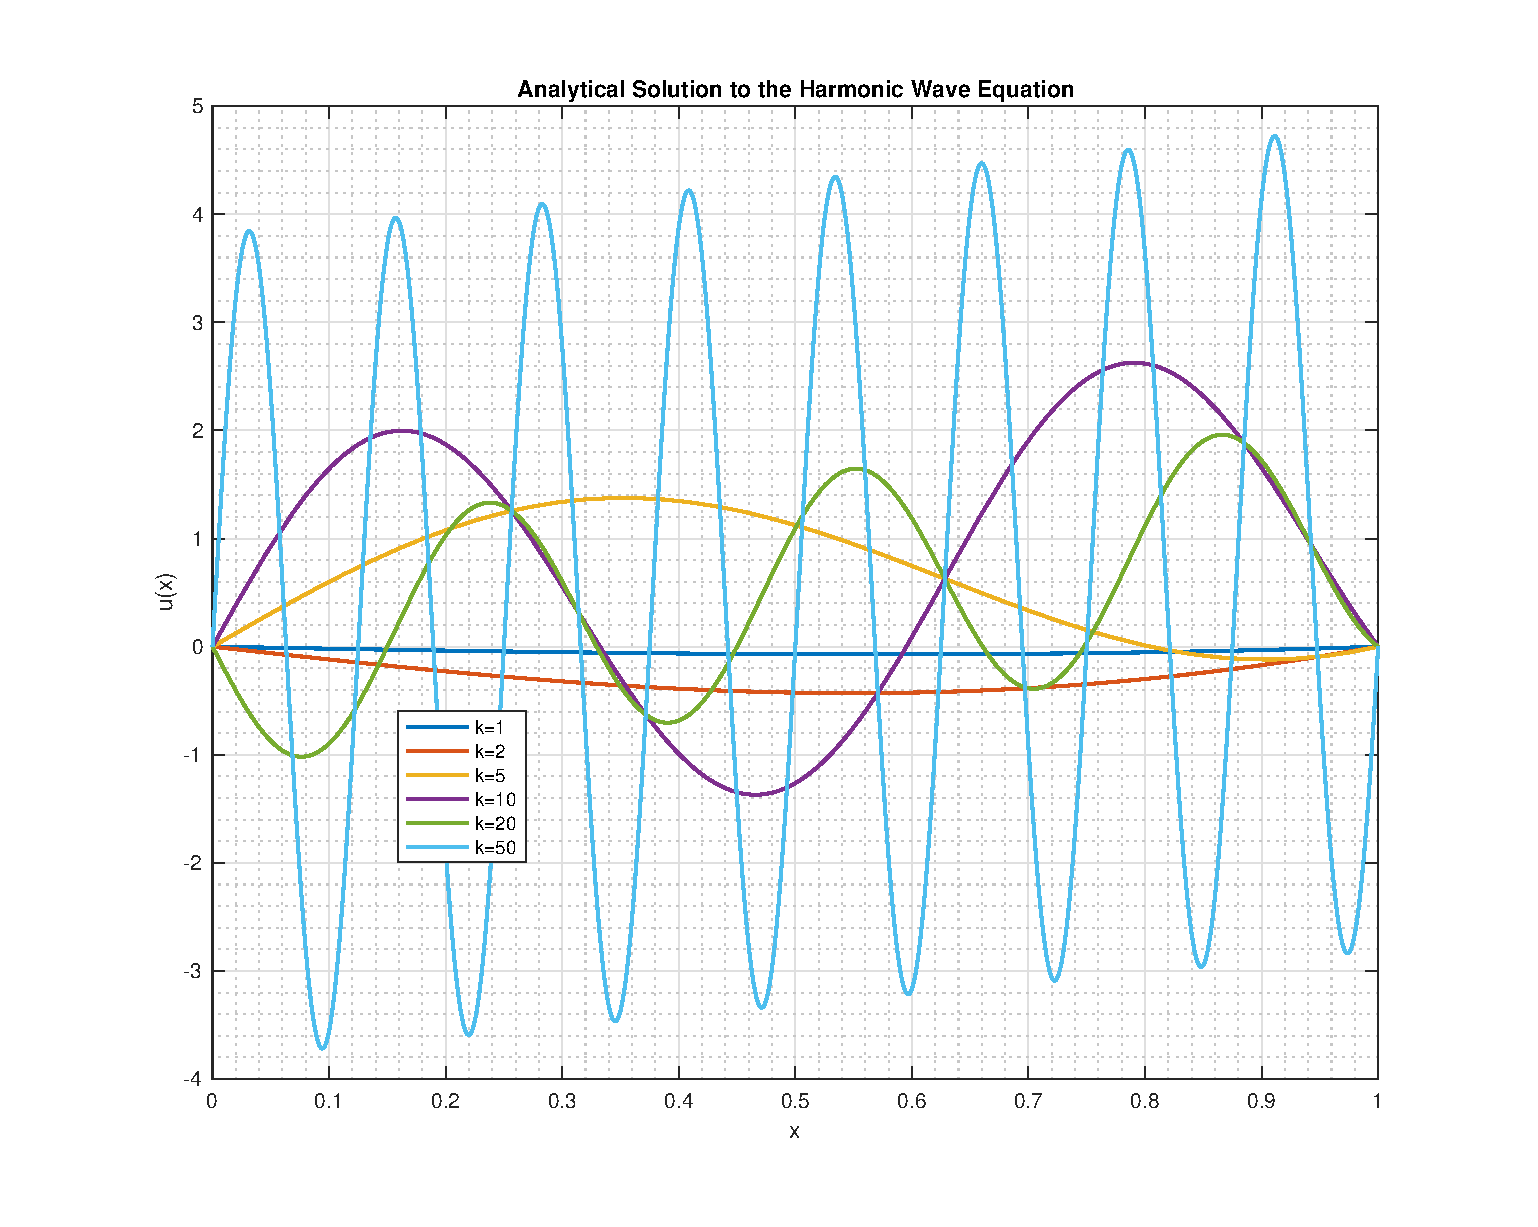
\includegraphics[width = 0.95\linewidth]{analytical_solution_harmonic_wave}
		\caption{Analytical Solution to the Harmonic Wave Equation for Values of $k$}
		\label{fig:analytical_harmonic}
	\end{center}
\end{figure}

\newpage

\subsection{1-D Convection-Diffusion Equation}

Previously, it was shown that for the one-dimensional second-order linear ordinary differential equation with specified boundary conditions (reproduced below), that $u(x)$ is a solution to the differential equation on $x \in [0, 1]$.
\begin{equation}
-u''(x)+cu'(x)=0 \qquad x \in [0, 1]
\end{equation}
\begin{equation}
u(0) = 0 \quad \textnormal{and} \quad u(1) = 1 
\end{equation}
\begin{equation}
u(x) = \frac{e^{cx}-1}{e^c-1}
\end{equation}

A plot of the analytical solution for values of $c$ is depicted in Figure \ref{fig:analytical_conv_diff}:
\begin{figure}[H]
	\begin{center}
		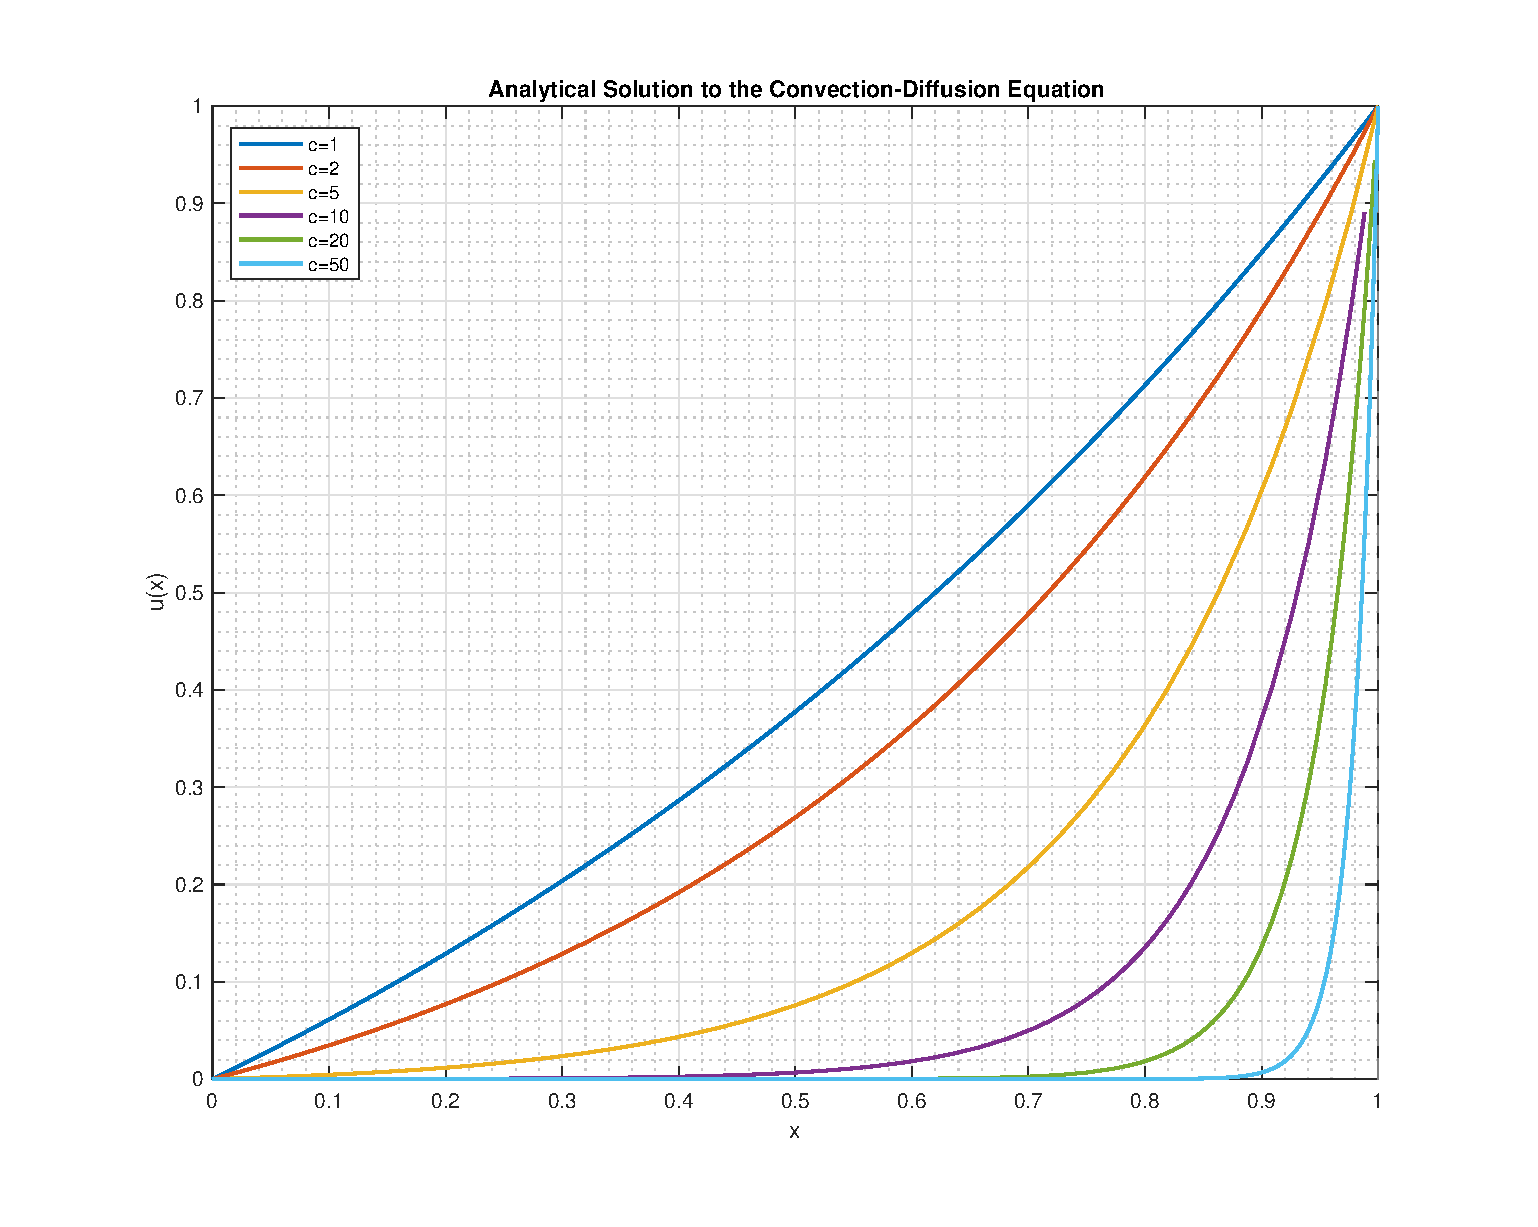
\includegraphics[width = 0.95\linewidth]{analytical_solution_convection_diffusion}
		\caption{Analytical Solution to the Convection-Diffusion Equation for Values of $c$}
		\label{fig:analytical_conv_diff}
	\end{center}
\end{figure}

\newpage

\subsection{2-D Orthotropic Diffusion Equation}

Previously, it was shown that for the two-dimensional second-order linear ordinary differential equation with specified boundary conditions (reproduced below), that $u(x,y)$ is a solution to the differential equation on $(x, y) \in [0, 1] \times [0, 1]$.
\begin{equation}
k^2\psder{u}{x} + \psder{u}{y} = 0 \qquad x,y \in [0, 1] \times [0, 1]
\end{equation}
\begin{equation}
\begin{split}
u(x, 0) = 0 \qquad \qquad \quad u(0, y) = 0  \\
u(x, 1) = \sin(\pi x) \qquad \; u(1, y) = 0
\end{split}
\end{equation}
\begin{equation}
u(x, y) = \frac{\sin(\pi x) \sinh(k\pi y)}{\sinh(k\pi)}
\end{equation}

A plot of the analytical solution for values of $k \in \{1, 10\}$ is depicted in Figures \ref{fig:2dortho1} and \ref{fig:2dortho2}:

\begin{figure}[H]
	\begin{center}
		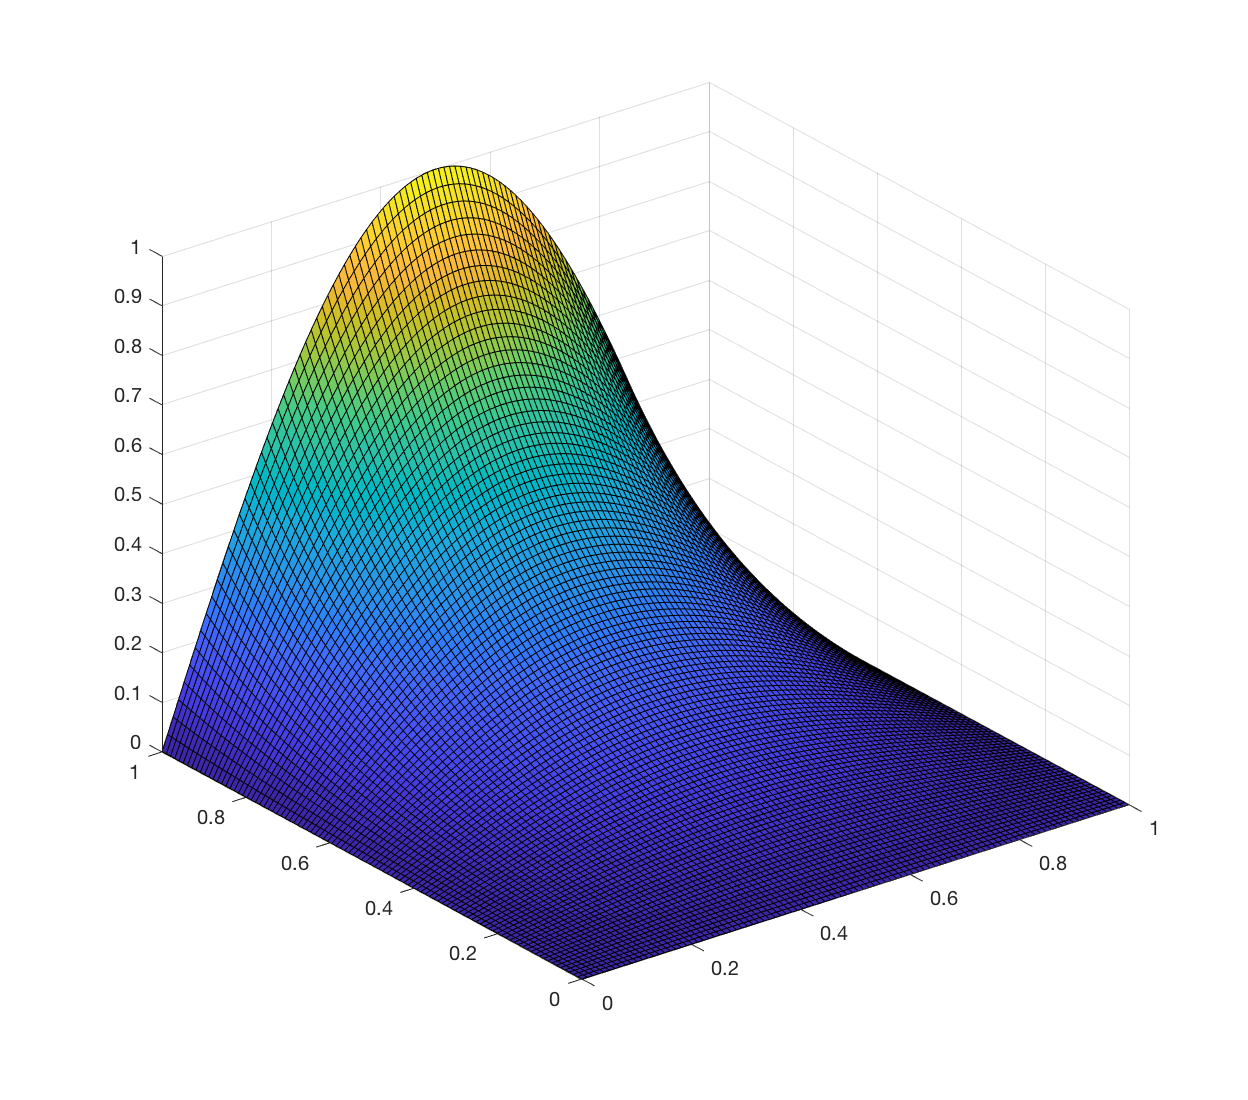
\includegraphics[width = 0.39\linewidth]{analytical_surface_k_1}
		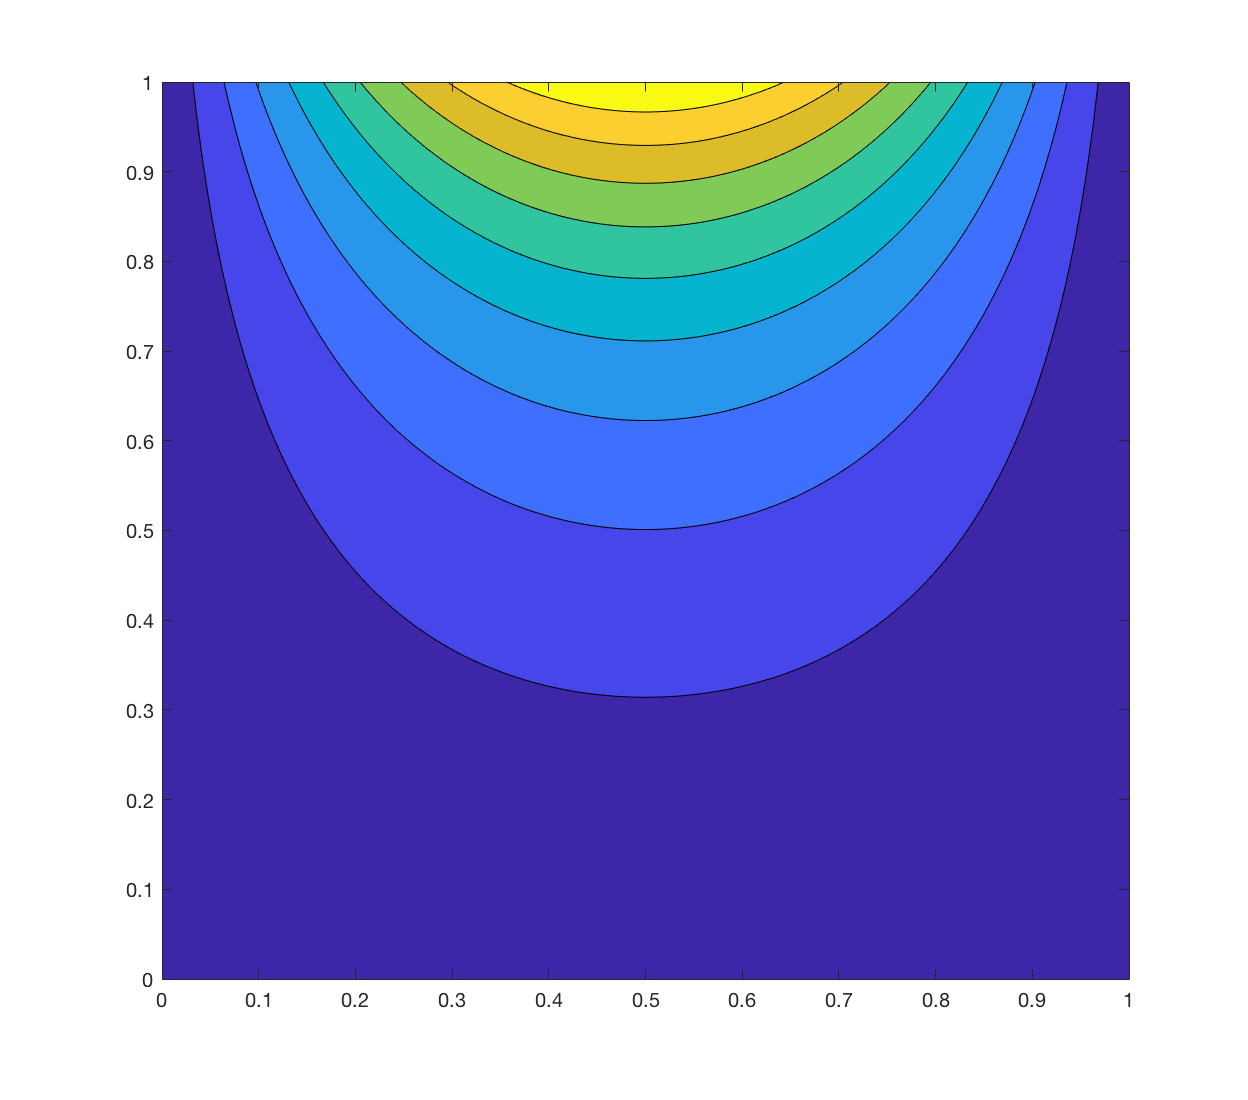
\includegraphics[width = 0.39\linewidth]{analytical_contour_k_1}
		\caption{Analytical Solution to the 2D Orthotropic Laplacian with $k = 1$}
		\label{fig:2dortho1}
	\end{center}
\end{figure}

\begin{figure}[H]
	\begin{center}
		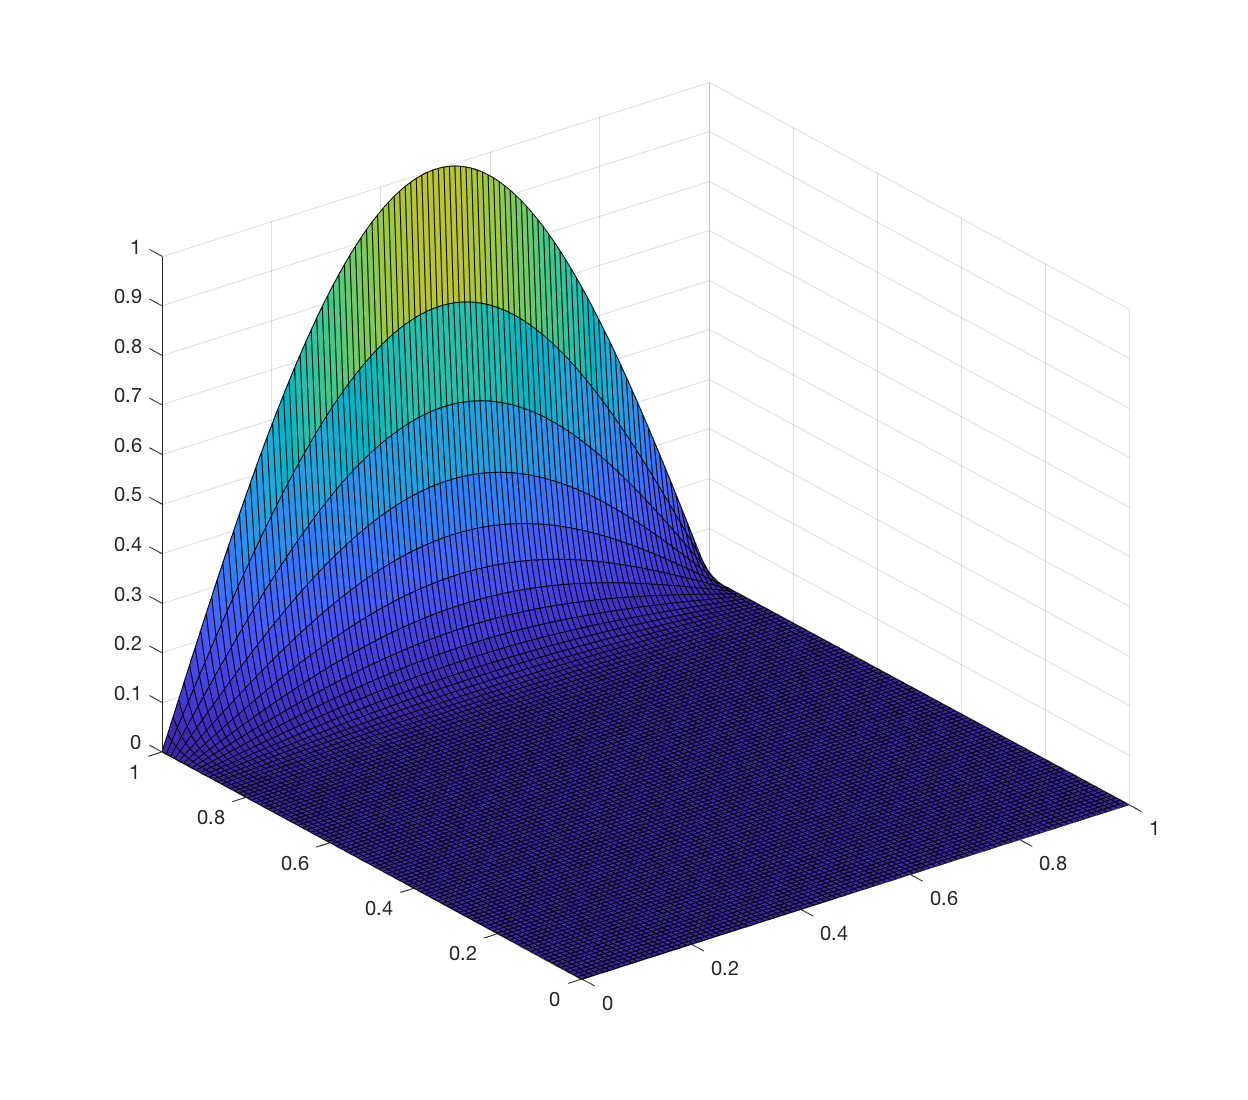
\includegraphics[width = 0.39\linewidth]{analytical_surface_k_10}
		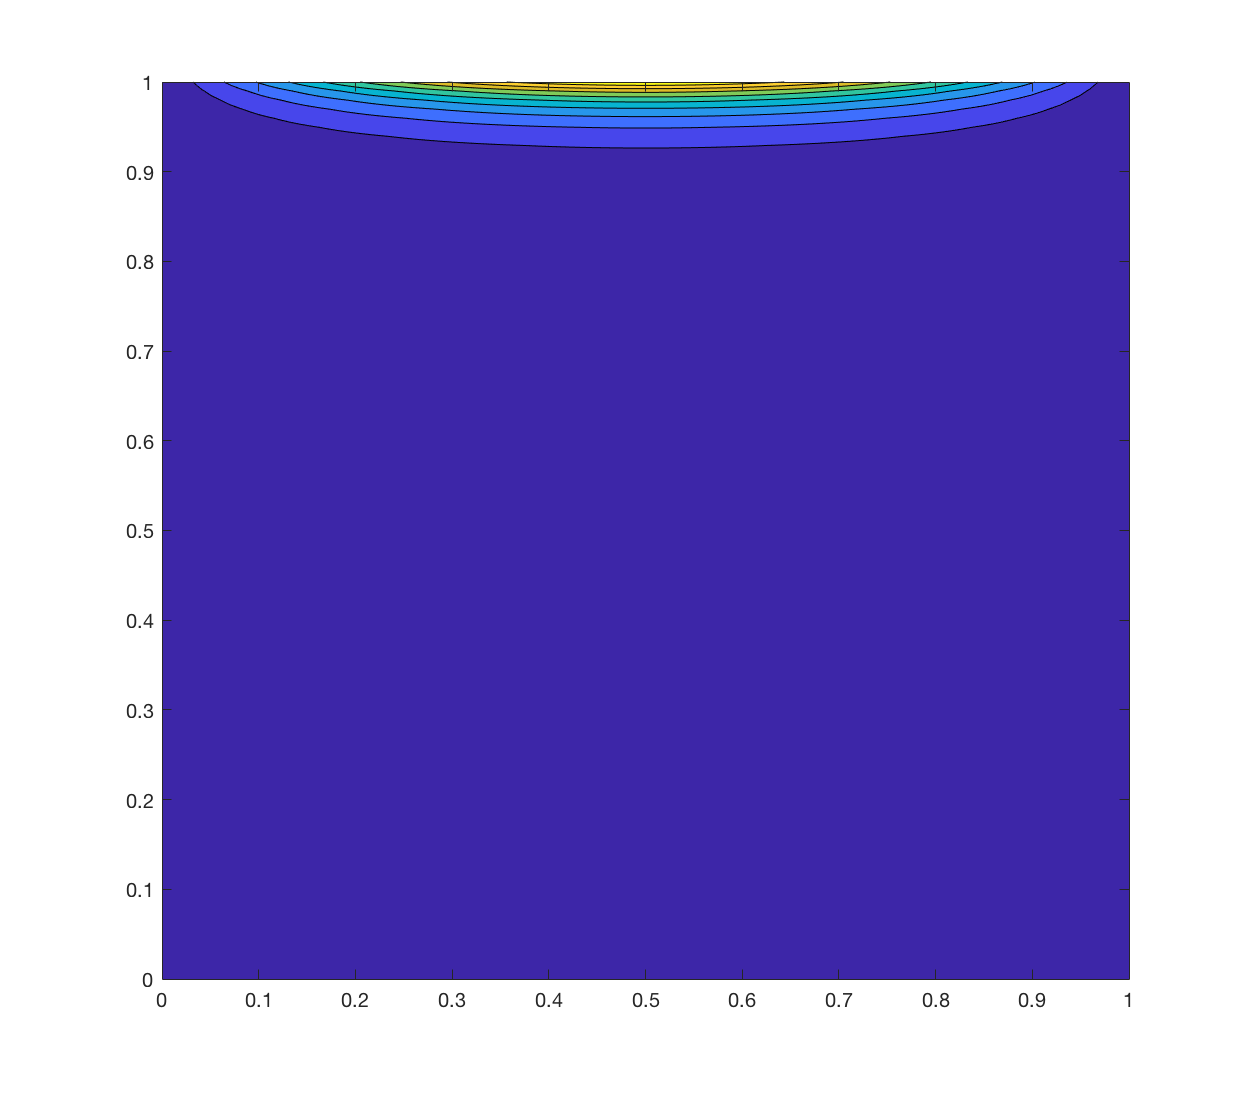
\includegraphics[width = 0.39\linewidth]{analytical_contour_k_10}
		\caption{Analytical Solution to the 2D Orthotropic Laplacian with $k = 10$}
		\label{fig:2dortho2}
	\end{center}
\end{figure}

\newpage

\section{Quantities of Interest}

\subsection{1-D Diffusion Equation}

The quantity of interest for the one-dimensional diffusion equation is the derivative at the right boundary, $u'(1)$. Previously, it was shown that the analytical solution of this derivative is given by:

\begin{equation}
u'(1) = 1 - k\coth(k)
\end{equation}

A table of the exact quantity of interest for the tested values of $k$ is included below (for $k \in \{20, 50\}$, error is less than machine epsilon, $\epsilon$):
\begin{table}[H]
	\caption{Analytical Solution to the Quantity of Interest for the 1-D Diffusion Equation for Values of $k$}
	\begin{tabular}{|c|c|}
		\hline 
		$\mathbf{k}$ & $\mathbf{u'(1)}$ \\ 
		\hline 
		1 & -0.313035 \\ 
		\hline 
		2 & -1.074629 \\ 
		\hline 
		5 & -4.000454 \\ 
		\hline 
		10 & -9.0000000412 \\ 
		\hline 
		20 & -19.000000000000000 \\ 
		\hline 
		50 & -49.000000000000000 \\ 
		\hline 
	\end{tabular}
\end{table} 

\subsection{1-D Harmonic Wave Equation}

The quantity of interest for the one-dimensional harmonic wave equation is the derivative at the right boundary, $u'(1)$. Previously, it was shown that the analytical solution of this derivative is given by:

\begin{equation}
u'(1) = 1 - k\cot(k)
\end{equation}

A table of the exact quantity of interest for the tested values of $k$ is included below:
\begin{table}[H]
	\caption{Analytical Solution to the Quantity of Interest for the 1-D Harmonic Wave Equation for Values of $k$}
	\begin{tabular}{|c|c|}
		\hline 
		$\mathbf{k}$ & $\mathbf{u'(1)}$ \\ 
		\hline 
		1 & 0.3579 \\ 
		\hline 
		2 & 1.9153 \\ 
		\hline 
		5 & 2.4790 \\ 
		\hline 
		10 & -14.4235 \\ 
		\hline 
		20 & -7.9399 \\ 
		\hline 
		50 & 184.8907 \\ 
		\hline 
	\end{tabular}
\end{table} 

\subsection{1-D Convection-Diffusion Equation}

The quantity of interest for the one-dimensional harmonic wave equation is the derivative at the right boundary, $u'(1)$. Previously, it was shown that the analytical solution of this derivative is given by:

\begin{equation}
u'(1) = \frac{ce^{c}}{e^c-1}
\end{equation}

A table of the exact quantity of interest for the tested values of $c$ is included below (for $c=50$, error is less than machine epsilon, $\epsilon$):
\begin{table}[H]
	\caption{Analytical Solution to the Quantity of Interest for the 1-D Convection-Diffusion Equation for Values of $c$}
	\begin{tabular}{|c|c|}
		\hline 
		$\mathbf{c}$ & $\mathbf{u'(1)}$ \\ 
		\hline 
		1 & 1.58198 \\ 
		\hline 
		2 & 2.31304 \\ 
		\hline 
		5 & 5.03392 \\ 
		\hline 
		10 & 10.00045 \\ 
		\hline 
		20 & 20.00000004 \\ 
		\hline 
		50 & 50.00000000 \\ 
		\hline 
	\end{tabular}
\end{table} 

\subsection{2-D Orthotropic Diffusion Equation}

The quantity of interest for the one-dimensional harmonic wave equation is the first partial derivative with respect to $y$ at the top central boundary, $u_y(\tfrac{1}{2}, 1)$. Previously, it was shown that the analytical solution of this derivative is given by:

\begin{equation}
u_y\left(\tfrac{1}{2},1\right) = k\pi \coth(k\pi)
\end{equation}

A table of the exact quantity of interest for the tested values of $k$ is included below:
\begin{table}[H]
	\caption{Analytical Solution to the Quantity of Interest for the 2-D Orthotropic Diffusion Equation for Values of $k$}
	\begin{tabular}{|c|c|}
		\hline 
		$\mathbf{k}$ & $\mathbf{u_y(\tfrac{1}{2}, 1)}$ \\ 
		\hline 
		1 & 3.1533 \\ 
		\hline 
		2 & 6.2832 \\ 
		\hline 
		5 & 15.7080 \\ 
		\hline 
		10 & 31.4159 \\ 
		\hline 
		20 & 62.8319 \\ 
		\hline 
		50 & 157.0796 \\ 
		\hline 
	\end{tabular}
\end{table} 

\newpage

\section{Numerical Methods}

\subsection{1-D Diffusion Equation}

\subsubsection{2nd-Order Central Difference Scheme - Exact Finite Difference Method}

Previously, it was shown that for the one-dimensional diffusion equation, the second-order discretization is:
\begin{equation}
\left(-1\right) u_{i-1} + \left(2 + k^2\Delta x^2\right) u_{i} + \left(-1\right) u_{i+1} = \left(k^2\Delta x^2 \right)x_i
\end{equation}

The solution of the diffusion equation was given earlier by:
\begin{equation}
u(x) = x - \frac{\sinh(kx)}{\sinh(k)}
\end{equation}
Replacing $k$ with $\bar{k}$ to represent the quasi-analytical finite difference coefficient, we arrive at:
\begin{equation}
u(x) = x - \frac{\sinh(\bar{k}x)}{\sinh(\bar{k})}
\end{equation}

Substituting this formula into the discretization and simplifying yields:
\begin{equation}
\bar{k} = \frac{1}{\Delta x} \cosh^{-1}\left(1+\frac{k^2\Delta x^2}{2}\right)
\end{equation}

\subsubsection{4th-Order Central Difference Scheme - Exact Finite Difference Method}

Previously, it was shown that for the one-dimensional diffusion equation, the fourth-order discretization is:
\begin{equation}
\left(-1 + \frac{k^2\Delta x^2}{12}\right) u_{i-1} + \left(2 + \frac{10 k^2\Delta x^2}{12}\right) u_{i} + \left(-1+ \frac{k^2\Delta x^2}{12}\right) u_{i+1} = \left(k^2\Delta x^2 \right)x_i
\end{equation}

The solution of the diffusion equation was given earlier by:
\begin{equation}
u(x) = x - \frac{\sinh(kx)}{\sinh(k)}
\end{equation}
Replacing $k$ with $\bar{k}$ to represent the quasi-analytical finite difference coefficient, we arrive at:
\begin{equation}
u(x) = x - \frac{\sinh(\bar{k}x)}{\sinh(\bar{k})}
\end{equation}

Substituting this formula into the discretization and simplifying yields:
\begin{equation}
\bar{k} = \frac{1}{\Delta x} \cosh^{-1}\left(\frac{2+\frac{10k^2\Delta x^2}{12}}{-2\left(-1+\frac{k^2\Delta x^2}{12}\right)}\right)
\end{equation}

\newpage

\subsection{1-D Harmonic Wave Equation}

\subsubsection{2nd-Order Central Difference Scheme - Exact Finite Difference Method}

Previously, it was shown that for the one-dimensional harmonic wave equation, the second-order discretization is:
\begin{equation}
\left(1\right) u_{i-1} + \left(-2 + k^2\Delta x^2\right) u_{i} + \left(1\right) u_{i+1} = \left(k^2\Delta x^2 \right)x_i
\end{equation}

The solution of the harmonic wave equation was given earlier by:
\begin{equation}
u(x) = x - \frac{\sin(kx)}{\sin(k)}
\end{equation}
Replacing $k$ with $\bar{k}$ to represent the quasi-analytical finite difference coefficient, we arrive at:
\begin{equation}
u(x) = x - \frac{\sin(\bar{k}x)}{\sin(\bar{k})}
\end{equation}

Substituting this formula into the discretization and simplifying yields:
\begin{equation}
\bar{k} = \frac{1}{\Delta x} \cosh^{-1}\left(1-\frac{k^2\Delta x^2}{2}\right)
\end{equation}

\subsubsection{4th-Order Central Difference Scheme - Exact Finite Difference Method}

Previously, it was shown that for the one-dimensional harmonic wave equation, the fourth-order discretization is:
\begin{equation}
\left(1 + \frac{k^2\Delta x^2}{12}\right) u_{i-1} + \left(-2 + \frac{10 k^2\Delta x^2}{12}\right) u_{i} + \left(1+ \frac{k^2\Delta x^2}{12}\right) u_{i+1} = \left(k^2\Delta x^2 \right)x_i
\end{equation}

The solution of the harmonic wave equation was given earlier by:
\begin{equation}
u(x) = x - \frac{\sin(kx)}{\sin(k)}
\end{equation}
Replacing $k$ with $\bar{k}$ to represent the quasi-analytical finite difference coefficient, we arrive at:
\begin{equation}
u(x) = x - \frac{\sin(\bar{k}x)}{\sin(\bar{k})}
\end{equation}

Substituting this formula into the discretization and simplifying yields:
\begin{equation}
\bar{k} = \frac{1}{\Delta x} \cosh^{-1}\left(\frac{-2+\frac{10k^2\Delta x^2}{12}}{-2\left(1+\frac{k^2\Delta x^2}{12}\right)}\right)
\end{equation}

\newpage

\subsection{1-D Convection-Diffusion Equation}

\subsubsection{2nd-Order Central Difference Scheme - Exact Finite Difference Method}

Previously, it was shown that for the one-dimensional convection-diffusion equation, the second-order discretization is:
\begin{equation}
\left(-1-\frac{c\Delta x}{2}\right)u_{i-1} + \left(2\right)u_{i} + \left(-1+\frac{c\Delta x}{2}\right)u_{i+1} = 0
\end{equation}

The solution of the convection-diffusion equation was given earlier by (here we exchange $c$ with $k$ for consistency):
\begin{equation}
u(x) = \frac{e^{kx}-1}{e^k-1}
\end{equation}
Replacing $k$ with $\bar{k}$ to represent the quasi-analytical finite difference coefficient, we arrive at:
\begin{equation}
u(x) = \frac{e^{\bar{k}x}-1}{e^{\bar{k}}-1}
\end{equation}

Substituting this formula into the discretization and simplifying yields:
\begin{equation}
\bar{k} = \frac{1}{\Delta x} \log \left(\frac{-1-\frac{k\Delta x^2}{2}}{-1+\frac{k\Delta x^2}{2}}\right)
\end{equation}

\subsubsection{4th-Order Central Difference Scheme - Exact Finite Difference Method}

Previously, it was shown that for the one-dimensional convection-diffusion equation, the fourth-order discretization is:
\begin{equation}
\left(-1-\frac{c\Delta x}{2}-\frac{c^2\Delta x^2}{12}\right)u_{i-1} + \left(2+\frac{c^2\Delta x^2}{6}\right)u_{i} + \left(-1+\frac{c\Delta x}{2}-\frac{c^2\Delta x^2}{12}\right)u_{i+1} = 0
\end{equation}

The solution of the convection-diffusion equation was given earlier by (here we exchange $c$ with $k$ for consistency):
\begin{equation}
u(x) = \frac{e^{kx}-1}{e^k-1}
\end{equation}
Replacing $k$ with $\bar{k}$ to represent the quasi-analytical finite difference coefficient, we arrive at:
\begin{equation}
u(x) = \frac{e^{\bar{k}x}-1}{e^{\bar{k}}-1}
\end{equation}

Substituting this formula into the discretization and simplifying yields:
\begin{equation}
\bar{k} = \frac{1}{\Delta x} \log\left(\frac{1+\frac{k\Delta x}{2}+\frac{k^2\Delta x^2}{12}}{1-\frac{k\Delta x}{2}+\frac{k^2\Delta x^2}{12}}\right)
\end{equation}

\subsection{2-D Orthotropic Diffusion Equation}

\subsubsection{2nd-Order Central Difference Scheme - Exact Finite Difference Method}

Previously, it was shown that for the two-dimensional orthotropic diffusion equation, the second-order discretization on a uniform mesh ($\Delta x = \Delta y$) is the 5-point stencil in $x$ and $y$:
\begin{table}[H]
	\begin{tabular}{ccc}
		& $u_{i, j+1}$ &  \\
		$k^2u_{i-1, j}$ & $-2(k^2+1)u_{i, j}$ & $k^2u_{i+1, j}$ \\
		& $u_{i, j-1}$ & 
	\end{tabular}
\end{table}

The solution of the orthotropic diffusion equation was given earlier by:
\begin{equation}
u(x, y) = \frac{\sin(\pi x) \sinh(k\pi y)}{\sinh(k\pi)}
\end{equation}
Replacing $k$ with $\bar{k}$ to represent the quasi-analytical finite difference coefficient, we arrive at:
\begin{equation}
u(x, y) = \frac{\sin(\pi x) \sinh(\bar{k}\pi y)}{\sinh(\bar{k}\pi)}
\end{equation}

Substituting this formula into the discretization and simplifying yields:
\begin{equation}
\bar{k} = \frac{1}{\pi\Delta x} \cosh^{-1} \left(k^2+1-k^2\cos(\pi\Delta x)\right)
\end{equation}

\subsubsection{4th-Order Central Difference Scheme - Exact Finite Difference Method}

Previously, it was shown that for the two-dimensional orthotropic diffusion equation, the second-order discretization on a uniform mesh ($\Delta x = \Delta y$) is the 9-point stencil in $x$ and $y$:
\begin{table}[H]
	\begin{tabular}{ccc}
		$\tfrac{1}{12}(k^2+1)u_{i-1, j+1}$ & $[1-\tfrac{2}{12}(k^2+1)]u_{i, j+1}$ & $\tfrac{1}{12}(k^2+1)u_{i+1, j+1}$  \\
		$[k^2-\tfrac{2}{12}(k^2+1)]u_{i-1, j}$ & $[(-2+\tfrac{4}{12})(k^2+1))]u_{i, j}$ & $[k^2-\tfrac{2}{12}(k^2+1)]u_{i+1, j}$ \\
		$\tfrac{1}{12}(k^2+1)u_{i-1, j-1}$ & $[1-\tfrac{2}{12}(k^2+1)]u_{i, j-1}$ & $\tfrac{1}{12}(k^2+1)u_{i+1, j-1}$
	\end{tabular}
\end{table}

We will use a simplification of the coefficients in the stencil for brevity:
\begin{table}[H]
	\begin{tabular}{ccc}
		$\alpha$ & $\beta$ & $\alpha$  \\
		$\gamma$ & $\delta$ & $\gamma$ \\
		$\alpha$ & $\beta$ & $\alpha$
	\end{tabular}
\end{table}

The solution of the orthotropic diffusion equation was given earlier by:
\begin{equation}
u(x, y) = \frac{\sin(\pi x) \sinh(k\pi y)}{\sinh(k\pi)}
\end{equation}
Replacing $k$ with $\bar{k}$ to represent the quasi-analytical finite difference coefficient, we arrive at:
\begin{equation}
u(x, y) = \frac{\sin(\pi x) \sinh(\bar{k}\pi y)}{\sinh(\bar{k}\pi)}
\end{equation}

Substituting this formula into the discretization and simplifying yields:
\begin{equation}
\bar{k} = \frac{1}{\pi\Delta x} \cosh^{-1} \left(\frac{-2\gamma\cos(\pi\Delta x) - \delta}{4\alpha\cos(\pi\Delta x)+2\beta}\right)
\end{equation}

\textit{Note: This equation works identically for the second-order stencil as long as the generalized coefficients are used.}

\newpage

\section{Convergence Analysis}

\subsection{Rate of Convergence Derivation}

Let the error for a particular mesh size $\Delta x$ be $E\left(\Delta x\right)$:
\begin{equation}
E\left(\Delta x\right) = C\left(\Delta x\right)^\beta
\end{equation}
Then for a smaller mesh size $\frac{\Delta x}{2}$ we have:
\begin{equation}
E\left(\frac{\Delta x}{2}\right) = C\left(\frac{\Delta x}{2}\right)^\beta
\end{equation}
Dividing the error at each mesh size and taking the logarithm:
\begin{equation}
\frac{E\left(\Delta x\right)}{E\left(\frac{\Delta x}{2}\right)} = \frac{C\left(\Delta x\right)^\beta}{C\left(\frac{\Delta x}{2}\right)^\beta} = 2^\beta
\end{equation}
\begin{equation}
\log\left[\frac{E\left(\Delta x\right)}{E\left(\frac{\Delta x}{2}\right)}\right] = \log(2^\beta)
\end{equation}
\begin{equation}
\log\left[\frac{E\left(\Delta x\right)}{E\left(\frac{\Delta x}{2}\right)}\right] = \beta \log(2)
\end{equation}
Rearranging for $\beta$ and simplifying:
\begin{equation}
\beta = \frac{1}{\log(2)} \left[\log\left(E\left(\Delta x\right)\right) - \log\left(E\left(\frac{\Delta x}{2}\right)\right)\right] 
\end{equation}
Denoting $E^*_{\Delta x} = \log\left(E\left(\Delta x\right)\right)$:
\begin{equation}
\mathbf{\beta = \frac{E^*_{\Delta x} - E^*_{\frac{\Delta x}{2}}}{\log (2)}}
\end{equation}

\newpage

\subsection{1-D Diffusion Equation}

\subsubsection{2nd-Order Central Difference Scheme}

\begin{figure}[H]
	\begin{center}
		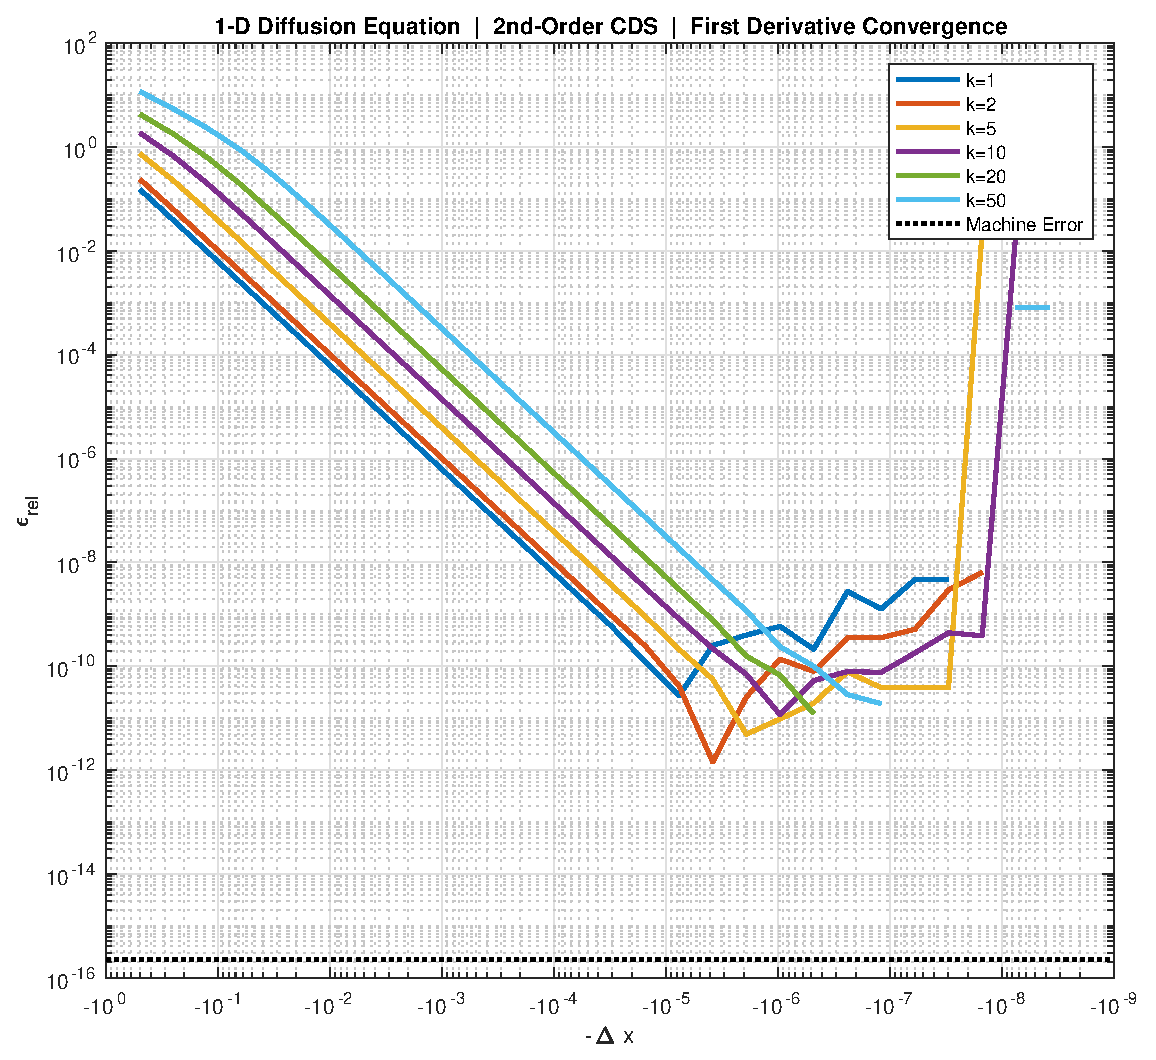
\includegraphics[width = 0.5\linewidth]{1ddiff2oconv}
		\caption{Rate of Convergence of $u'(1)$ for 2nd-Order CDS for the 1-D Diffusion Equation for Several Values of $k$ Using Exact FDM}	
	\end{center}
\end{figure}

\begin{figure}[H]
	\begin{center}
		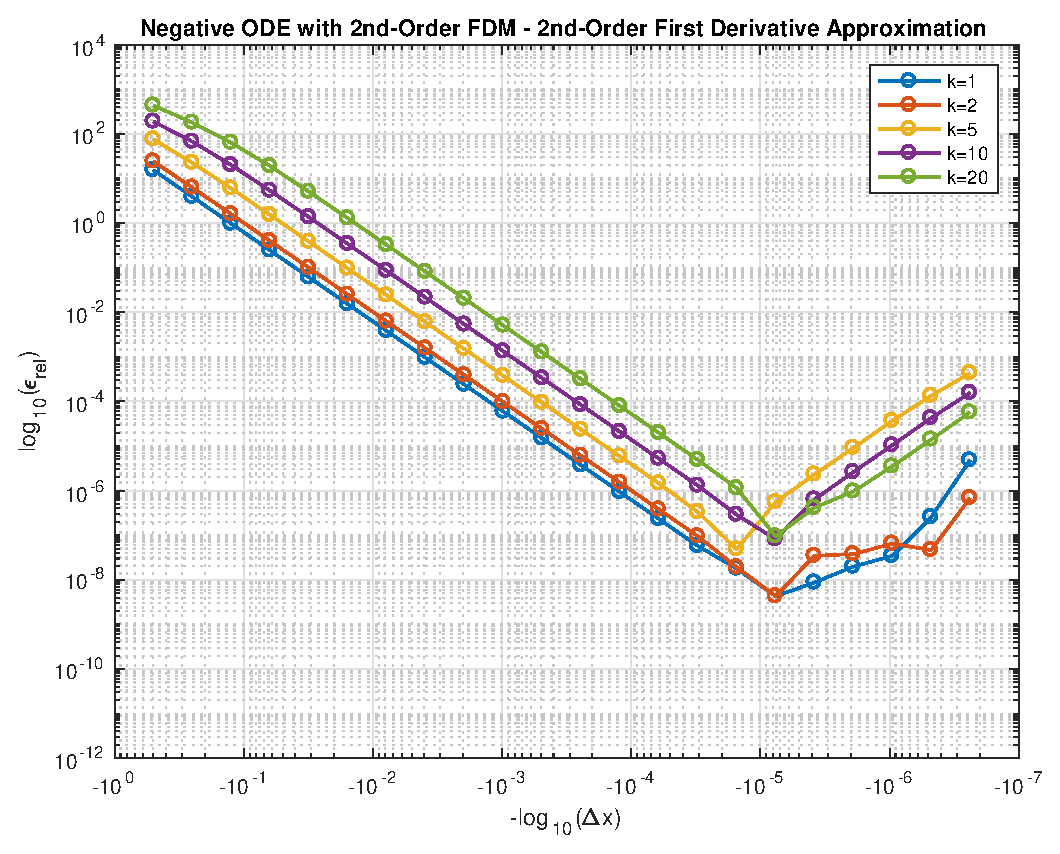
\includegraphics[width = 0.5\linewidth]{negative_ode_order_2_fd_order_2}
		\caption{Rate of Convergence of $u'(1)$ for 2nd-Order CDS for the 1-D Diffusion Equation for Several Values of $k$ Using Algebraic System FDM}	
	\end{center}
\end{figure}

\subsubsection{4th-Order Central Difference Scheme}

\begin{figure}[H]
	\begin{center}
		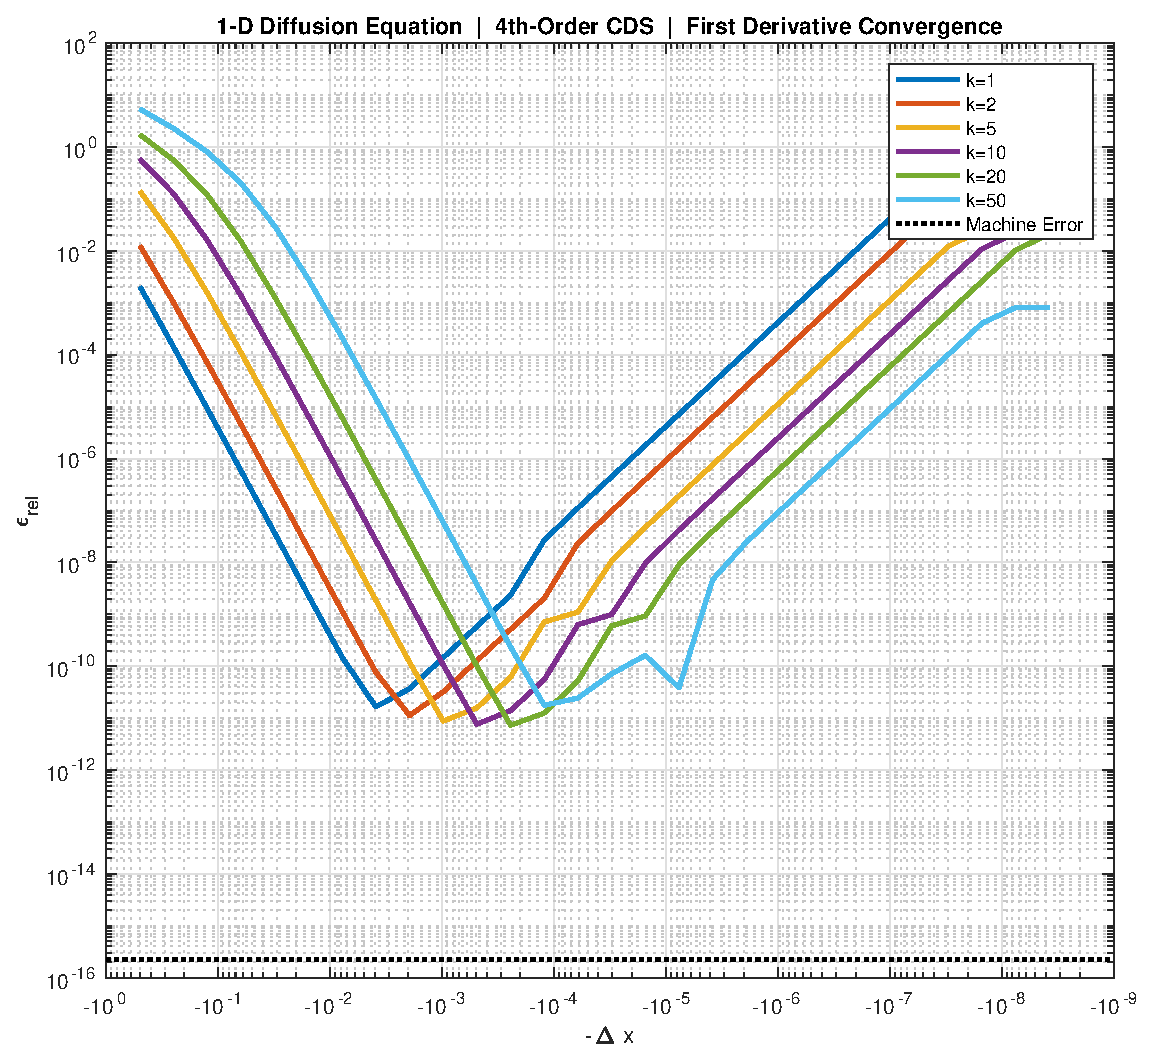
\includegraphics[width = 0.5\linewidth]{1ddiff4oconv}
		\caption{Rate of Convergence of $u'(1)$ for 4th-Order CDS for the 1-D Diffusion Equation for Several Values of $k$ Using Exact FDM}	
	\end{center}
\end{figure}

\begin{figure}[H]
	\begin{center}
		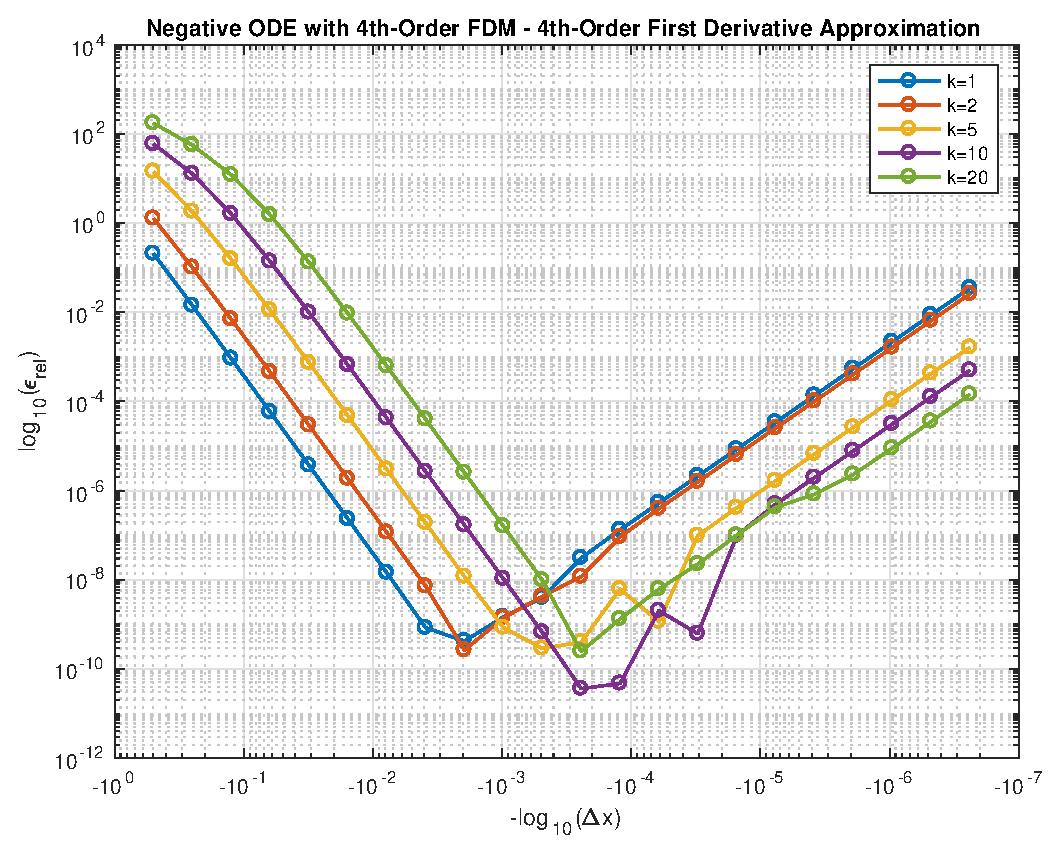
\includegraphics[width = 0.5\linewidth]{negative_ode_order_4_fd_order_4}
		\caption{Rate of Convergence of $u'(1)$ for 4th-Order CDS for the 1-D Diffusion Equation for Several Values of $k$ Using Algebraic System FDM}	
	\end{center}
\end{figure}

\subsection{1-D Harmonic Wave Equation}

\subsubsection{2nd-Order Central Difference Scheme}

\begin{figure}[H]
	\begin{center}
		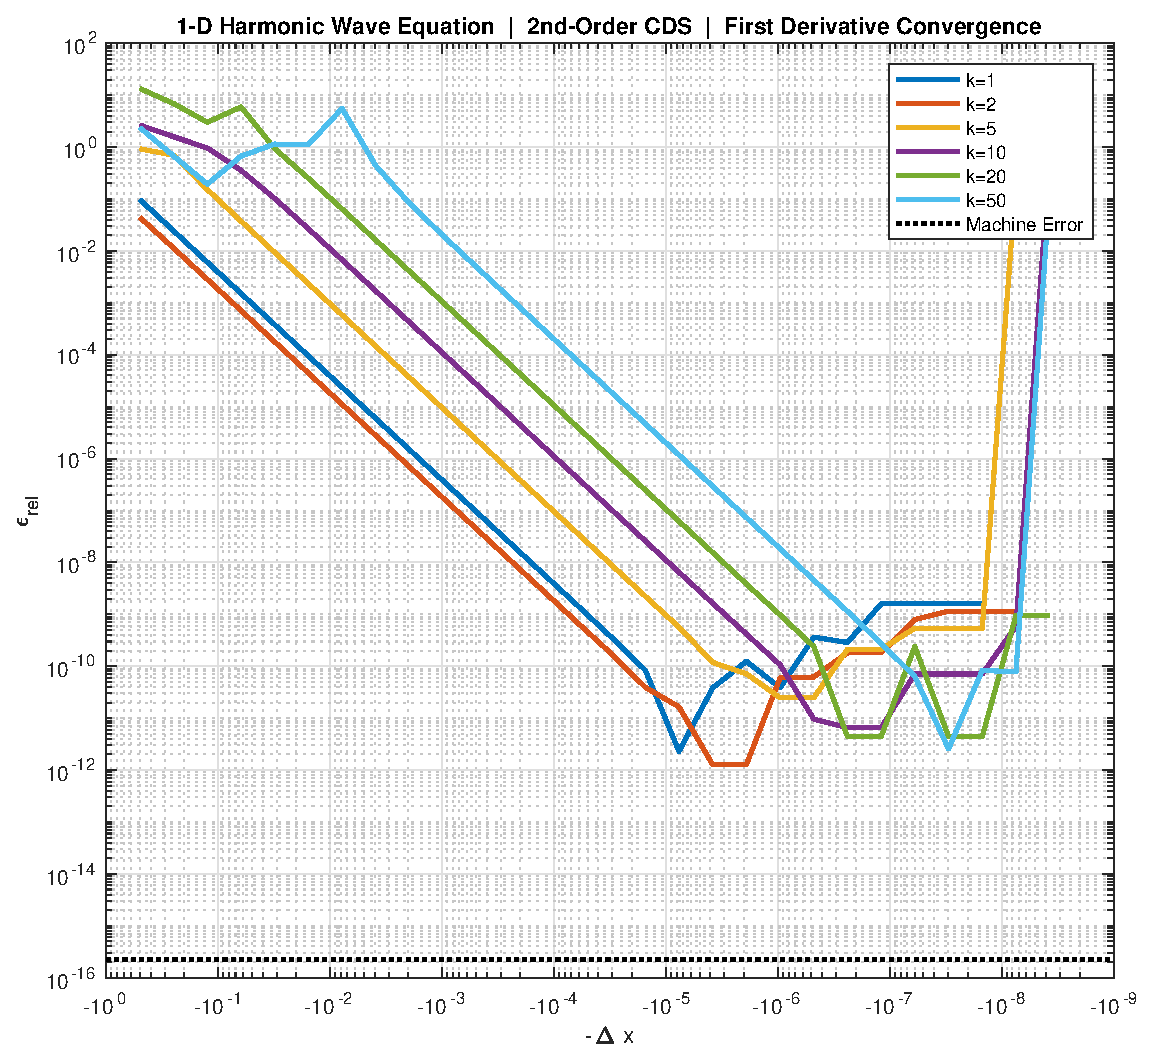
\includegraphics[width = 0.5\linewidth]{1dwave2oconv}
		\caption{Rate of Convergence of $u'(1)$ for 2nd-Order CDS for the 1-D Harmonic Wave Equation for Several Values of $k$ Using Exact FDM}	
	\end{center}
\end{figure}

\begin{figure}[H]
	\begin{center}
		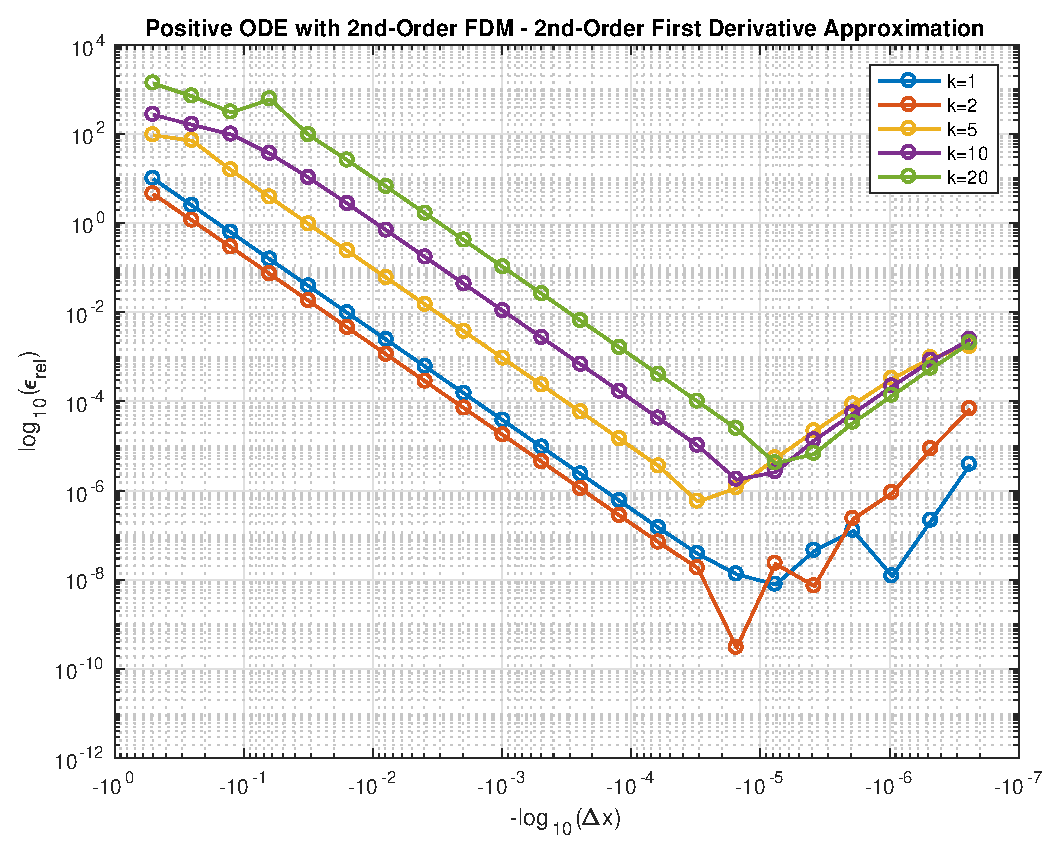
\includegraphics[width = 0.5\linewidth]{positive_ode_order_2_fd_order_2}
		\caption{Rate of Convergence of $u'(1)$ for 2nd-Order CDS for the 1-D Harmonic Wave Equation for Several Values of $k$ Using Algebraic System FDM}	
	\end{center}
\end{figure}

\subsubsection{4th-Order Central Difference Scheme}

\begin{figure}[H]
	\begin{center}
		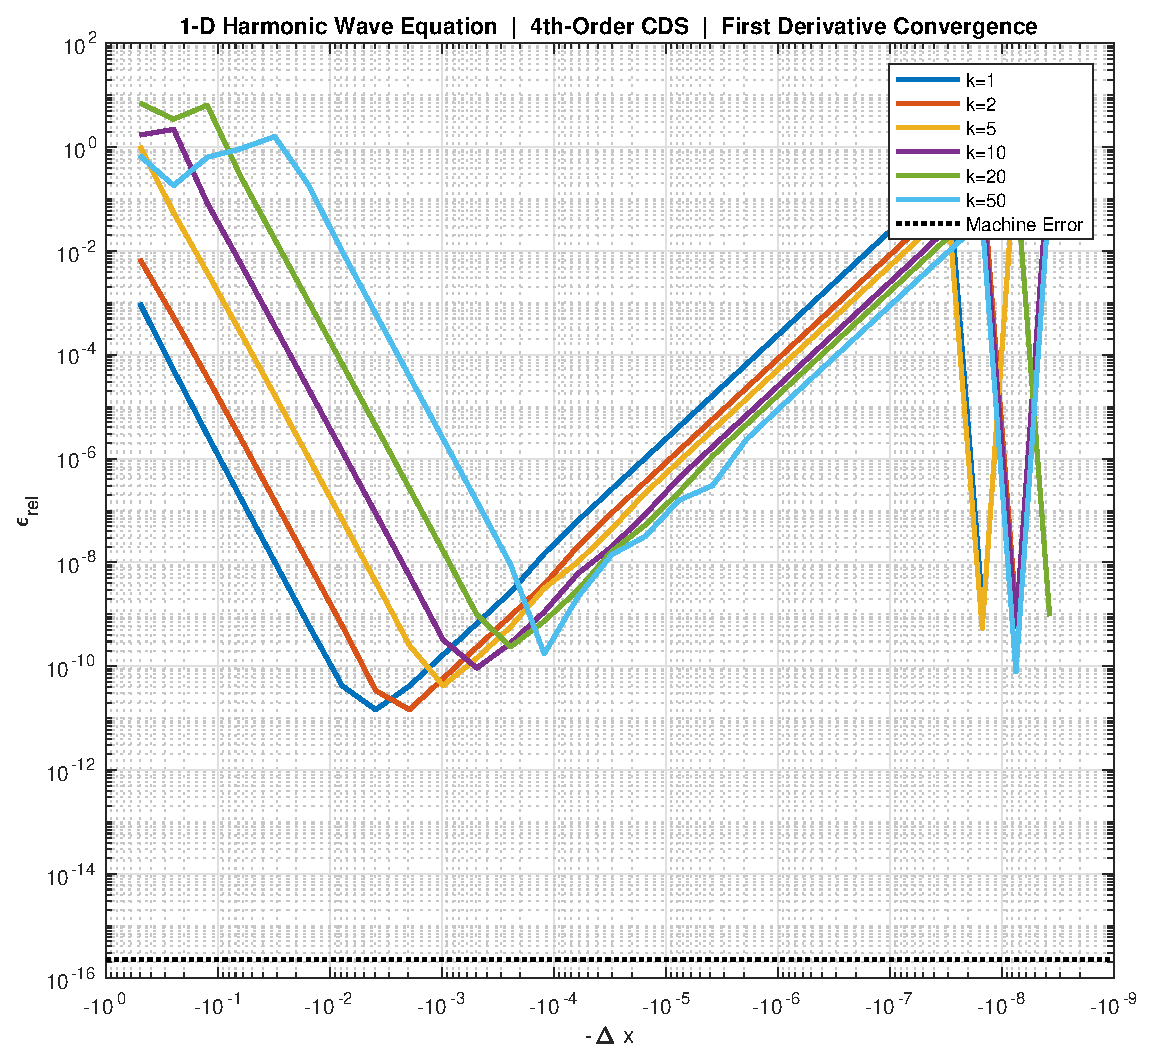
\includegraphics[width = 0.5\linewidth]{1dwave4oconv}
		\caption{Rate of Convergence of $u'(1)$ for 4th-Order CDS for the 1-D Harmonic Wave Equation for Several Values of $k$ Using Exact FDM}	
	\end{center}
\end{figure}

\begin{figure}[H]
	\begin{center}
		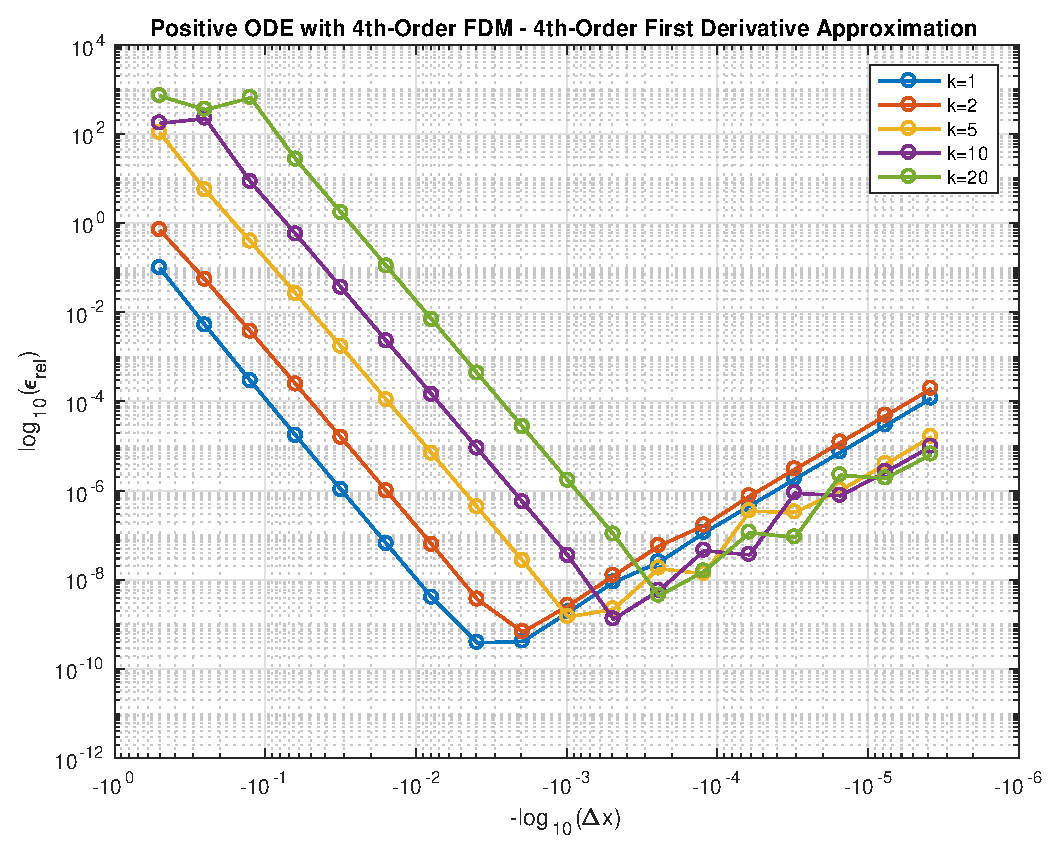
\includegraphics[width = 0.5\linewidth]{positive_ode_order_4_fd_order_4}
		\caption{Rate of Convergence of $u'(1)$ for 4th-Order CDS for the 1-D Harmonic Wave Equation for Several Values of $k$ Using Algebraic System FDM}	
	\end{center}
\end{figure}

\subsection{1-D Convection-Diffusion Equation}

\subsubsection{2nd-Order Central Difference Scheme}

\begin{figure}[H]
	\begin{center}
		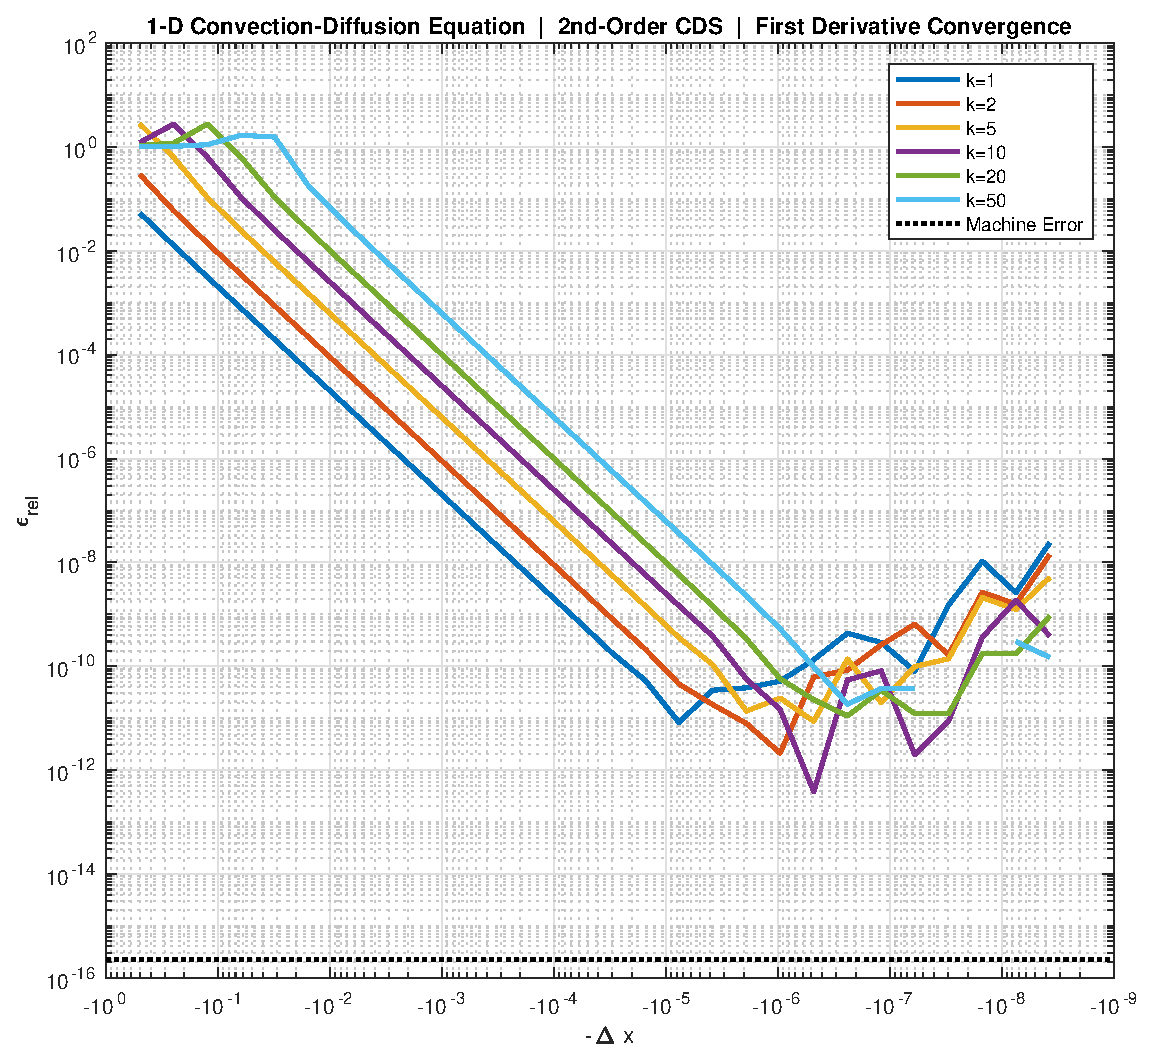
\includegraphics[width = 0.5\linewidth]{1dconv2oconv}
		\caption{Rate of Convergence of $u'(1)$ for 2nd-Order CDS for the 1-D Convection-Diffusion Equation for Several Values of $k$ Using Exact FDM}	
	\end{center}
\end{figure}

\begin{figure}[H]
	\begin{center}
		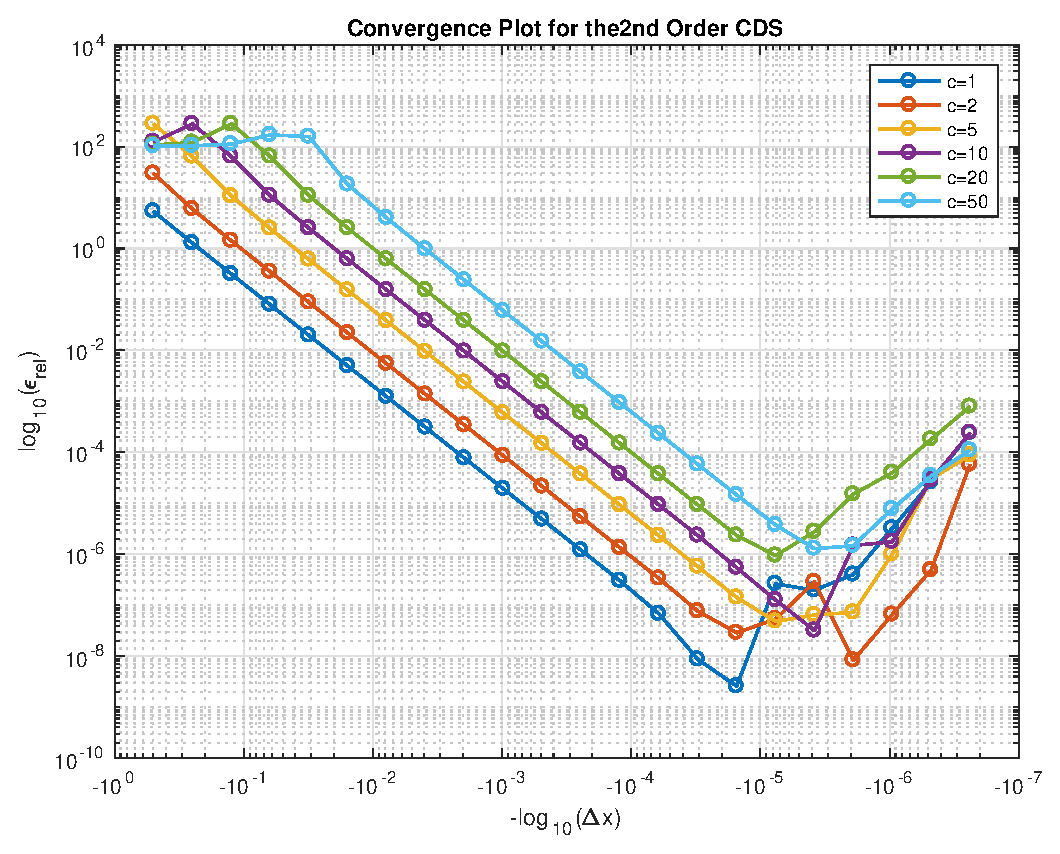
\includegraphics[width = 0.5\linewidth]{convergence_2nd_order_cds}
		\caption{Rate of Convergence of $u'(1)$ for 2nd-Order CDS for the 1-D Convection-Diffusion Equation for Several Values of $k$ Using Algebraic System FDM}	
	\end{center}
\end{figure}

\subsubsection{4th-Order Central Difference Scheme}

\begin{figure}[H]
	\begin{center}
		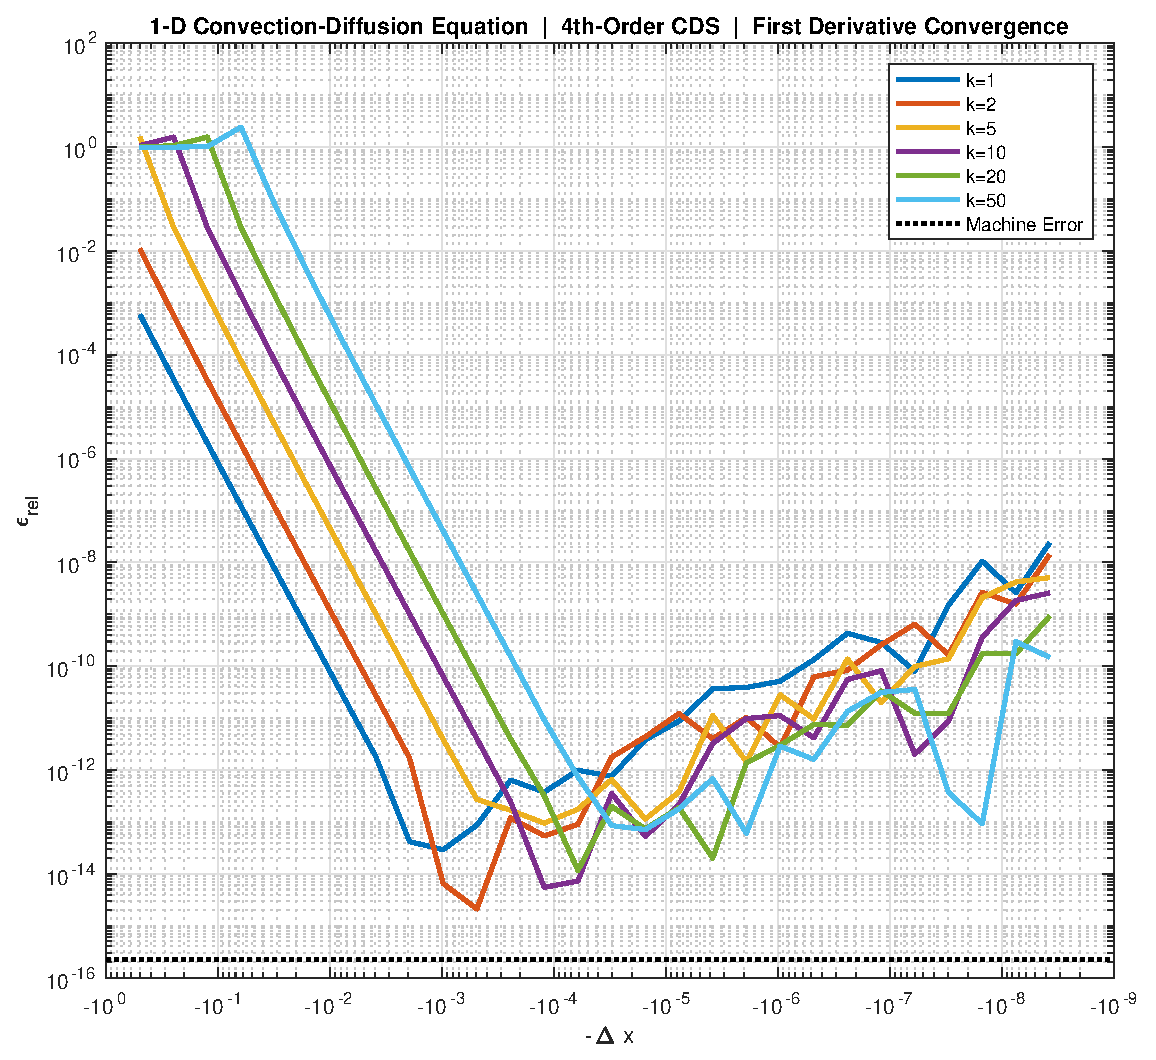
\includegraphics[width = 0.5\linewidth]{1dconv4oconv}
		\caption{Rate of Convergence of $u'(1)$ for 4th-Order CDS for the 1-D Convection-Diffusion Equation for Several Values of $k$ Using Exact FDM}	
	\end{center}
\end{figure}

\begin{figure}[H]
	\begin{center}
		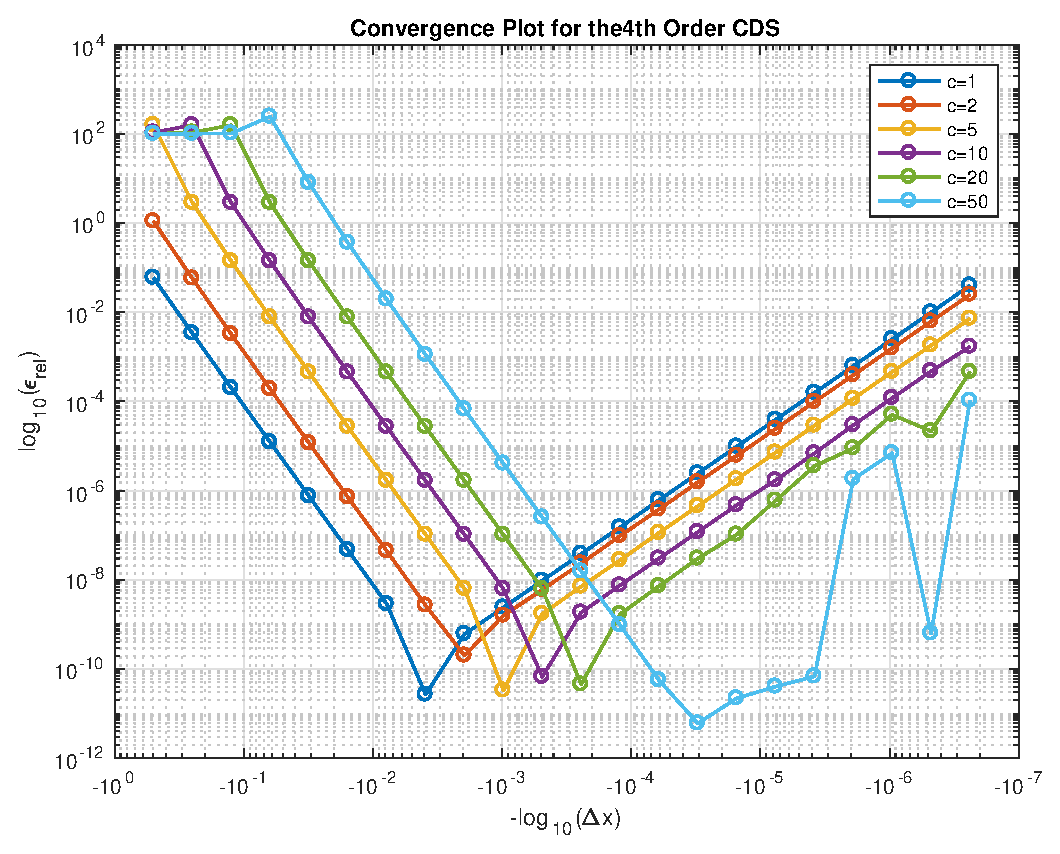
\includegraphics[width = 0.5\linewidth]{convergence_4th_order_cds}
		\caption{Rate of Convergence of $u'(1)$ for 4th-Order CDS for the 1-D Convection-Diffusion Equation for Several Values of $k$ Using Algebraic System FDM}	
	\end{center}
\end{figure}

\subsection{2-D Orthotropic Diffusion Equation}

\subsubsection{2nd-Order Central Difference Scheme}

\begin{figure}[H]
	\begin{center}
		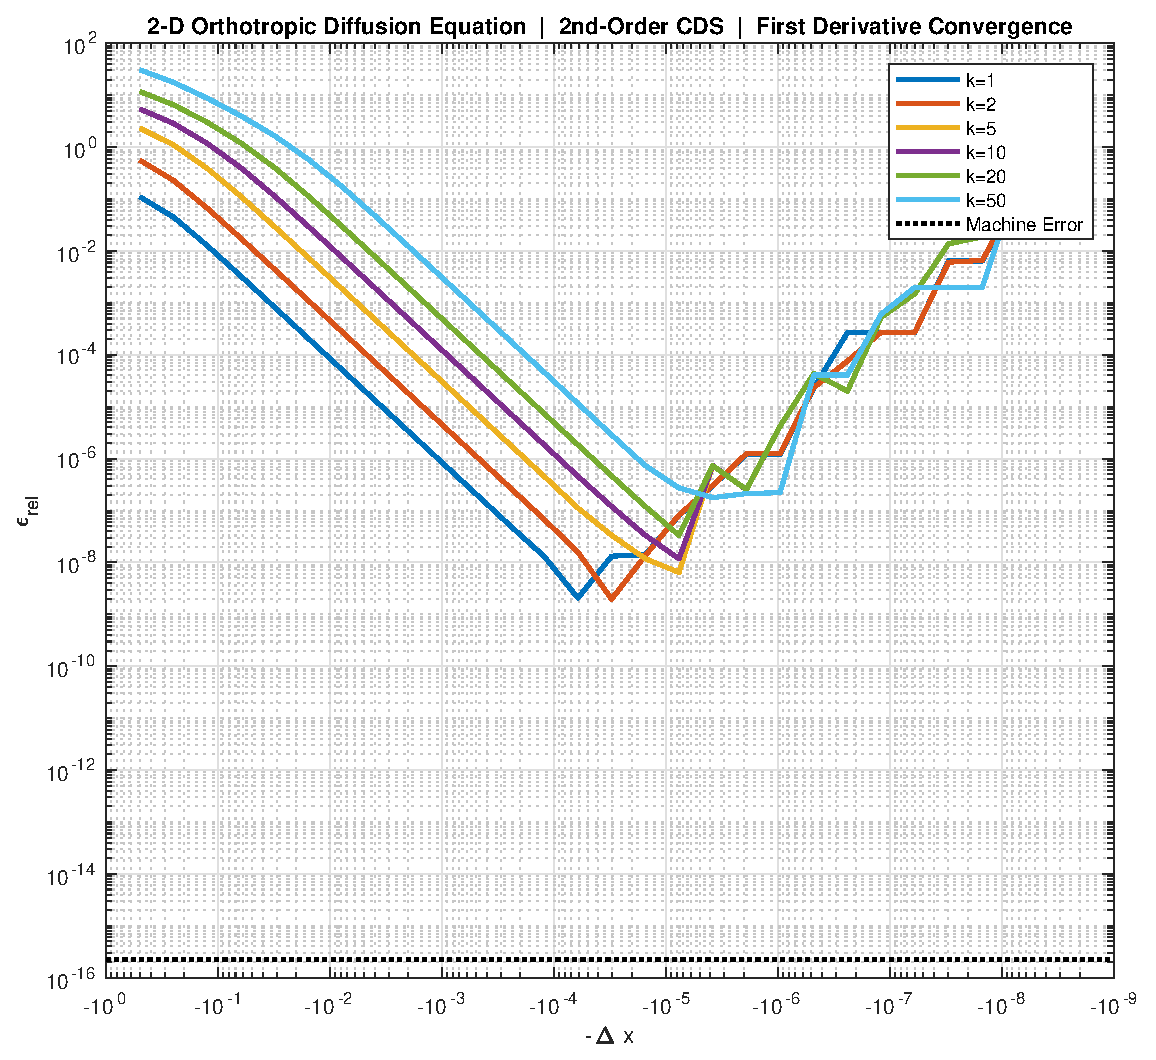
\includegraphics[width = 0.5\linewidth]{2ddiff2oconv}
		\caption{Rate of Convergence of $u_y(\tfrac{1}{2},1)$ for 2nd-Order CDS for the 2-D Orthotropic Diffusion Equation for Several Values of $k$ Using Exact FDM}	
	\end{center}
\end{figure}

\begin{figure}[H]
	\begin{center}
		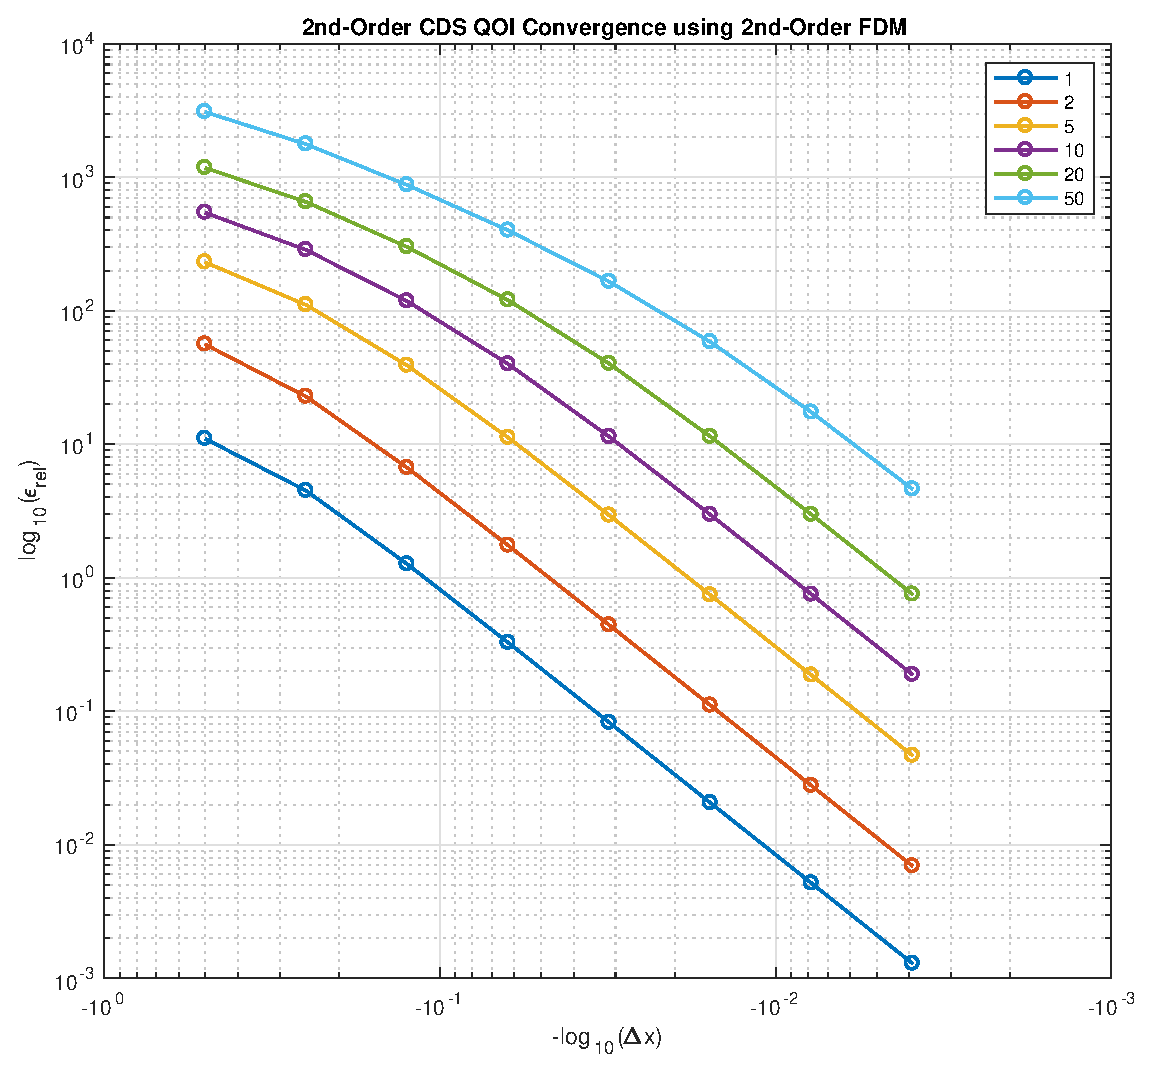
\includegraphics[width = 0.5\linewidth]{order_2_u_y_fdm}
		\caption{Rate of Convergence of $u_y(\tfrac{1}{2},1))$ for 2nd-Order CDS for the 2-D Orthotropic Diffusion Equation for Several Values of $k$ Using Algebraic System FDM}	
	\end{center}
\end{figure}

\subsubsection{4th-Order Central Difference Scheme}

\begin{figure}[H]
	\begin{center}
		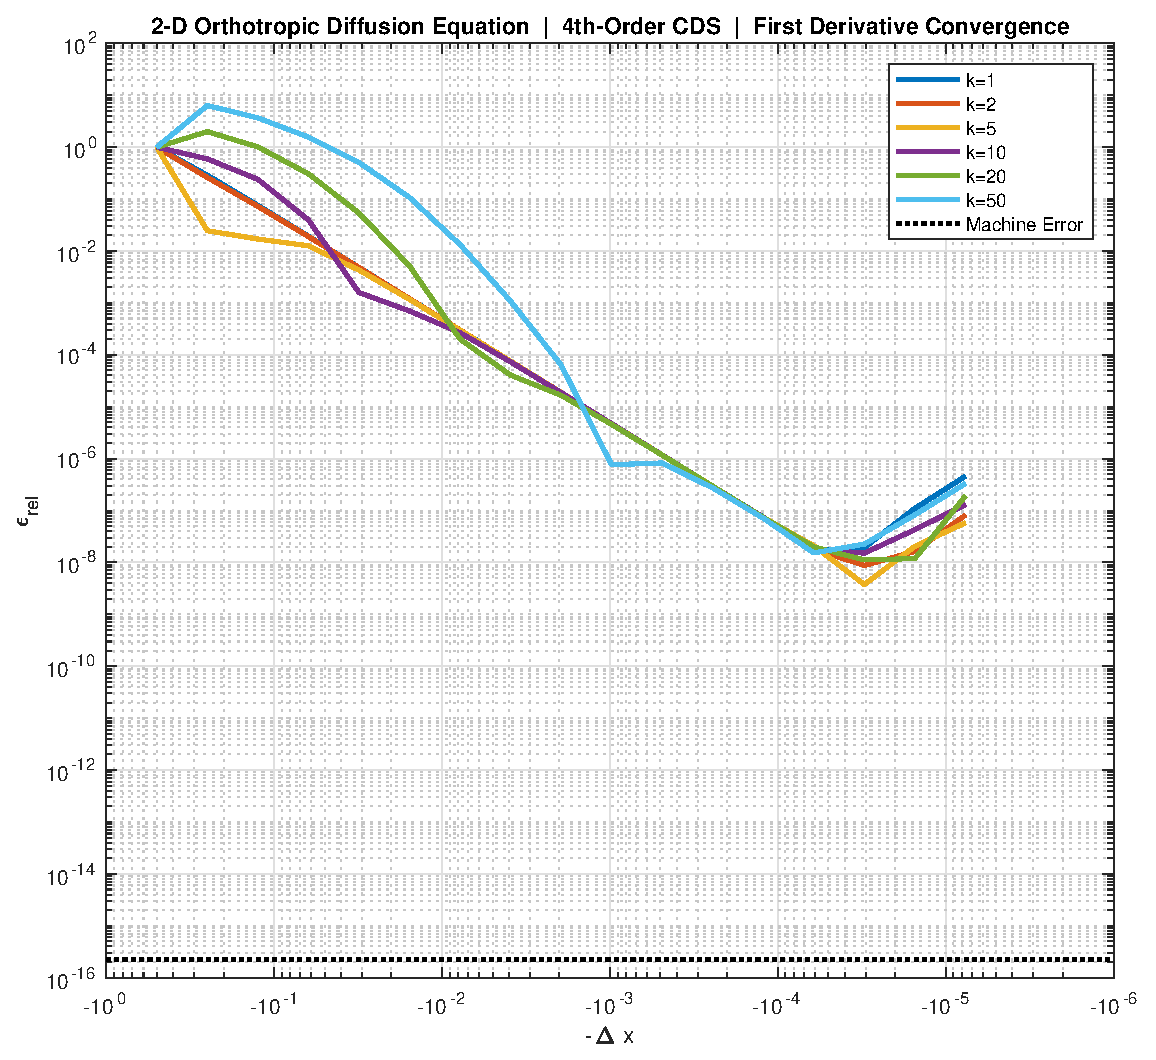
\includegraphics[width = 0.5\linewidth]{2ddiff4oconv}
		\caption{Rate of Convergence of $u_y(\tfrac{1}{2},1)$ for 4th-Order CDS for the 2-D Orthotropic Diffusion Equation for Several Values of $k$ Using Exact FDM}	
	\end{center}
\end{figure}

\begin{figure}[H]
	\begin{center}
		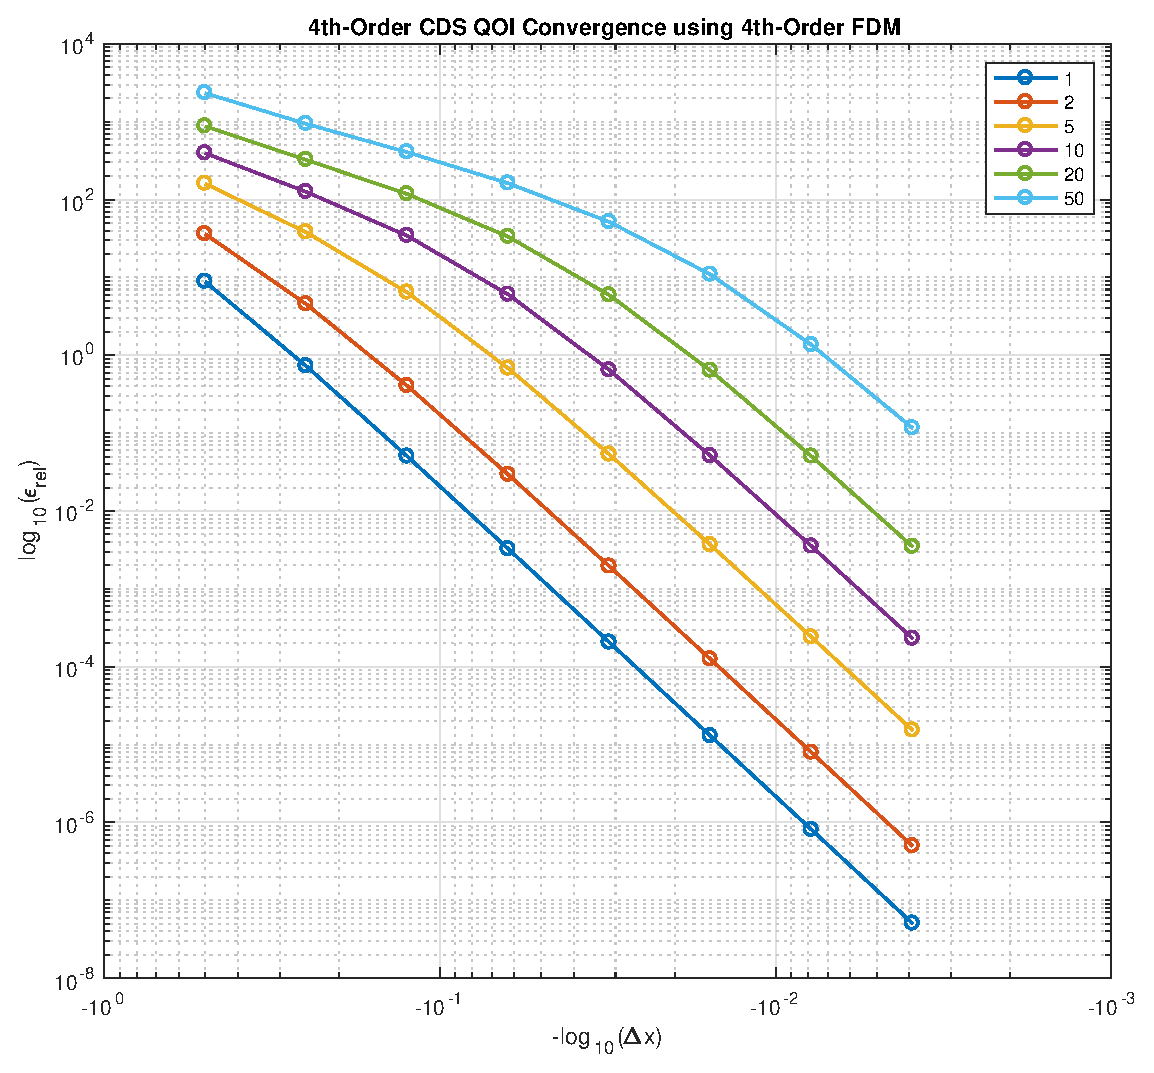
\includegraphics[width = 0.5\linewidth]{order_4_u_y_fdm}
		\caption{Rate of Convergence of $u_y(\tfrac{1}{2},1)$ for 4th-Order CDS for the 2-D Orthotropic Diffusion Equation for Several Values of $k$ Using Algebraic System FDM}	
	\end{center}
\end{figure}

\newpage

\section{Discussion}

In all cases, it is easy to see that the exact finite difference method solution approach is much simpler than the linear algebraic solution approach. The latter requires the simultaneous solution of all grid points (in 2-D and 3-D this realization becomes much more computationally intensive), while the former allows the calculation of each grid point individually, once the quasi-analytical coefficient is determined. In general, this means that the exact finite difference method approach allows for significantly faster computation times, smaller computational memory allocation, and reduced roundoff error.

\vspace{10 pt}

If a solution in the exact finite difference method exists for a particular differential equation, then variants also exist in similar form, as shown with the 2-D orthotropic diffusion equation.

\vspace{10 pt}

For the 1-D diffusion equation, meshes were computed down to $\Delta x = 2^{-28}$. The error in the 2nd-order scheme is roughly lower than that computed with the algebraic form of the finite difference equations, but the solution was able to be computed for much smaller mesh sizes. The error in the 4th-order scheme is roughly lower than that computed with the algebraic form of the finite difference equations, but again the solution was able to be computed for much smaller mesh sizes. For both methods, the asymptotic rate of convergence was strictly the order of the method ($\beta = 2$, $\beta = 4$).

\vspace{10 pt}

For the 1-D harmonic wave equation, meshes were computed down to $\Delta x = 2^{-28}$. The error in the 2nd-order scheme is much lower than that computed with the algebraic form of the finite difference equations and approaches $10^{-12}$. The error in the 4th-order scheme is roughly lower than that computed with the algebraic form of the finite difference equations. In both cases, the solution was able to be computed for much smaller mesh sizes. For both methods, the asymptotic rate of convergence was strictly the order of the method ($\beta = 2$, $\beta = 4$).

\vspace{10 pt}

For the 1-D convection-diffusion equation, meshes were computed down to $\Delta x = 2^{-28}$. The error in the 2nd-order scheme is much lower than that computed with the algebraic form of the finite difference equations and approaches $10^{-12}$. The error in the 4th-order scheme is much lower than that computed with the algebraic form of the finite difference equations and approaches $10^{-15}$ -- near machine epsilon, $\varepsilon$! In both cases, the solution was able to be computed for much smaller mesh sizes. For both methods, the asymptotic rate of convergence was strictly the order of the method ($\beta = 2$, $\beta = 4$).

\vspace{10 pt}

For the 2-D orthotropic diffusion equation, meshes were computed down to $\Delta x = 2^{-28}$ for the 2nd-order scheme and $\Delta x = 2^{-17}$. The error in the 2nd-order scheme advances significantly below that computed with the algebraic form of the finite difference equations and approaches $10^{-9}$. With maximum computing power for the algebraic form of the finite difference equations, computations could only be computed down to $\Delta x = 2^{-8}$. The error in the 4th-order scheme is roughly lower than that computed with the algebraic form of the finite difference equations and approaches $10^{-9}$. For both methods, the asymptotic rate of convergence was strictly the order of the method ($\beta = 2$, $\beta = 4$).

\vspace{10 pt}

\hrule

\vspace{10 pt}

In general, the difference between the convergence of the equations is due in large part to their form and stability. The 1-D diffusion equation and the 1-D harmonic wave equation have largely different convergence properties -- one solution is hyperbolic trigonometric and the other solution is purely trigonometric. Additionally, the 1-D convection-diffusion equation implemented with a central difference scheme is unstable for small mesh sizes, but extremely stable once the Peclet condition is satisfied.

\vspace{10 pt}

There are significant changes from the 1-D equations to the 2-D orthotropic diffusion equation. It is seen that for the second-order method, the derivative can be extracted \textit{explicitly}, but for the fourth-order method, the derivative must be extracted \textit{implicitly}. This shows some of the limitations of this method. The aim of the exact FDM is to avoid the extensive computation resources of the algebraic solution method, and the higher-order method makes this increasingly difficult. Regardless, the results were still able to be extended to much smaller mesh sizes with minimal computational effort.

\vspace{10 pt}

\textbf{In general, convergence rates using the exact finite difference method were equivalent to the convergence rates using the algebraic finite difference method, but were achieved at a much lower cost.}

\newpage

\appendix

\section{MATLAB Code}

\subsection{fp\_1d\_diffusion.m}

\begin{lstlisting}
clear all; close all; clc

meshOrder   = 1:28;
meshDx      = (1/2).^meshOrder;

order = 2;

ufdm = sparse([]);
uexact = sparse([]);

index = 0;

for k = [1 2 5 10 20 50]

index = index + 1;

for dx = meshDx

clear ufdm

if order == 2

kbar = 1 / dx * acosh(1 + k^2*dx^2/2);

%             x = 0:dx:1;
%             ufdm(-log(dx)/log(2), 1:1/dx+1) = x - sinh(kbar*x)/sinh(kbar);
%             uxfdm = -ufdm(-log(dx)/log(2), end-1) / dx - dx * k^2 / 2;

ufdm = 1-dx - sinh(kbar*(1-dx))/sinh(kbar);
uxfdm = -ufdm / dx - dx * k^2 / 2;

uxexact = 1 - k*coth(k);

elseif order == 4

kbar = 1 / dx * acosh((2+10*k^2*dx^2/12) / (-2*(-1+k^2*dx^2/12)));

%             x = 0:dx:1;
%             ufdm(-log(dx)/log(2), 1:1/dx+1) = x - sinh(kbar*x)/sinh(kbar);
%             uxfdm = 1 / (1 + dx^2 * k^2 / 6) * (-ufdm(-log(dx)/log(2), end-1) / dx - dx * k^2 / 2 + ...
%                     dx^2 * k^2 / 6 - dx^3 * k^4 / 24);

ufdm = 1-dx - sinh(kbar*(1-dx))/sinh(kbar);
uxfdm = 1 / (1 + dx^2 * k^2 / 6) * (-ufdm / dx - dx * k^2 / 2 + ...
dx^2 * k^2 / 6 - dx^3 * k^4 / 24);        

uxexact = 1 - k*coth(k);

end

err(-log(dx)/log(2)) = abs((uxfdm - uxexact) / uxexact);

end

uxerr(index, :) = err;

end

figure
hold on
set(gcf, 'Position', [1 1 624 550])

for i = 1:index
plot(-meshDx, uxerr(i, :), 'linewidth', 2);
end
plot([-10^0 -10^-9], [eps eps], 'k:', 'linewidth', 2)
legend('k=1', 'k=2', 'k=5', 'k=10', 'k=20', 'k=50', 'Machine Error')
xlabel('-\Delta x'); ylabel('\epsilon_r_e_l')
title('1-D Diffusion Equation  |  First Derivative Convergence')

set(gca, 'xscale', 'log')
set(gca, 'yscale', 'log')
grid on; grid minor;
box on;
\end{lstlisting}

\subsection{fp\_1d\_wave.m}

\begin{lstlisting}
clear all; close all; clc

meshOrder   = 1:28;
meshDx      = (1/2).^meshOrder;

order = 2;

ufdm = sparse([]);
uexact = sparse([]);

index = 0;

for k = [1 2 5 10 20 50]

index = index + 1;

for dx = meshDx

clear ufdm

if order == 2

kbar = 1 / dx * acos(1 - k^2*dx^2/2);

%             x = 0:dx:1;
%             ufdm(-log(dx)/log(2), 1:1/dx+1) = x - sin(kbar*x)/sin(kbar);
%             uxfdm = -ufdm(-log(dx)/log(2), end-1) / dx + dx * k^2 / 2; 

ufdm = 1-dx - sin(kbar*(1-dx))/sin(kbar);
uxfdm = -ufdm / dx + dx * k^2 / 2; 

uxexact = 1 - k*cot(k);

elseif order == 4

kbar = 1 / dx * acos((-2+10*k^2*dx^2/12) / (-2*(1+k^2*dx^2/12)));

%             x = 0:dx:1;
%             ufdm(-log(dx)/log(2), 1:1/dx+1) = x - sin(kbar*x)/sin(kbar);
%             uxfdm = 1 / (1 - dx^2 * k^2 / 6) * (-ufdm(-log(dx)/log(2), end-1) / dx + dx * k^2 / 2 - ...
%                     dx^2 * k^2 / 6 - dx^3 * k^4 / 24);

ufdm = 1-dx - sin(kbar*(1-dx))/sin(kbar);
uxfdm = 1 / (1 - dx^2 * k^2 / 6) * (-ufdm / dx + dx * k^2 / 2 - ...
dx^2 * k^2 / 6 - dx^3 * k^4 / 24);

uxexact = 1 - k*cot(k);

end

err(-log(dx)/log(2)) = abs((uxfdm - uxexact) / uxexact);

end

uxerr(index, :) = err;

end

figure
hold on
set(gcf, 'Position', [1 1 624 550])

for i = 1:index
plot(-meshDx, uxerr(i, :), 'linewidth', 2);
end
plot([-10^0 -10^-9], [eps eps], 'k:', 'linewidth', 2)
legend('k=1', 'k=2', 'k=5', 'k=10', 'k=20', 'k=50', 'Machine Error')
xlabel('-\Delta x'); ylabel('\epsilon_r_e_l')
title('1-D Harmonic Wave Equation  |  First Derivative Convergence')

set(gca, 'xscale', 'log')
set(gca, 'yscale', 'log')
grid on; grid minor;
box on;
\end{lstlisting}

\subsection{fp\_1d\_convection.m}

\begin{lstlisting}
clear all; close all; clc

meshOrder   = 1:28;
meshDx      = (1/2).^meshOrder;

order = 4;

ufdm = sparse([]);
uexact = sparse([]);

index = 0;

for k = [1 2 5 10 20 50]

index = index + 1;

for dx = meshDx

clear ufdm 

if order == 2

kbar = 1 / dx * log(((-2-k*dx)/(-2+k*dx)));

%            x = 0:dx:1;
%            ufdm(-log(dx)/log(2), 1:1/dx+1) = (exp(kbar*x) - 1) / (exp(kbar) - 1);
%            uxfdm = (1 - k*dx/2)^-1 * (1 - ufdm(-log(dx)/log(2), end-1)) / dx;

ufdm = (exp(kbar*(1-dx)) - 1) / (exp(kbar) - 1);
uxfdm = (1 - k*dx/2)^-1 * (1 - ufdm) / dx;

uxexact = k*exp(k) / (exp(k) - 1);

elseif order == 4

kbar = 1 / dx * log((-1 - k*dx/2 - k^2*dx^2/12)/(-1 + k*dx/2 - k^2*dx^2/12));

%            x = 0:dx:1;
%            ufdm(-log(dx)/log(2), 1:1/dx+1) = (exp(kbar*x) - 1) / (exp(kbar) - 1);
%            uxfdm = (1 -k*dx/2 + k^2*dx^2/6 - k^3*dx^3/24)^-1 * ...
%                 (1 - ufdm(-log(dx)/log(2), end-1)) / dx;

ufdm = (exp(kbar*(1-dx)) - 1) / (exp(kbar) - 1);
uxfdm = (1 -k*dx/2 + k^2*dx^2/6 - k^3*dx^3/24)^-1 * ...
(1 - ufdm) / dx;

uxexact = k*exp(k) / (exp(k) - 1);

end

err(-log(dx)/log(2)) = abs((uxfdm - uxexact) / uxexact);

end

uxerr(index, :) = err;

end

figure
hold on
set(gcf, 'Position', [1 1 624 550])

for i = 1:index
plot(-meshDx, uxerr(i, :), 'linewidth', 2);
end
plot([-10^0 -10^-9], [eps eps], 'k:', 'linewidth', 2)
legend('k=1', 'k=2', 'k=5', 'k=10', 'k=20', 'k=50', 'Machine Error')
xlabel('-\Delta x'); ylabel('\epsilon_r_e_l')
title('1-D Convection-Diffusion Equation  |  First Derivative Convergence')

set(gca, 'xscale', 'log')
set(gca, 'yscale', 'log')
grid on; grid minor;
box on;
\end{lstlisting}

\newpage

\subsection{fp\_2d\_diffusion.m}

\begin{lstlisting}
clear all; close all; clc

meshOrder   = 1:28;
meshDx      = (1/2).^meshOrder;

order = 2;

ufdm = sparse([]);
uexact = sparse([]);

index = 0;

for k = [1 2 5 10 20 50]

index = index + 1;

for dx = meshDx

if order == 2

kbar = 1/(pi*dx) * acosh(k^2+1-k^2*cos(pi*dx));

ufdmcenter = sin(pi*1/2)*sinh(kbar*pi*1)/sinh(kbar*pi);
ufdmright = sin(pi*(1/2+dx))*sinh(kbar*pi*1)/sinh(kbar*pi);
ufdmleft = sin(pi*(1/2-dx))*sinh(kbar*pi*1)/sinh(kbar*pi);
ufdmlower = sin(pi*1/2)*sinh(kbar*pi*(1-dx))/sinh(kbar*pi);

uyfdm = 1 / dx * ((1+k^2)*ufdmcenter - ufdmlower - k^2/2*ufdmleft - k^2/2*ufdmright);
uyexact = k*pi*coth(k*pi);

elseif order == 4

alpha = 1/12*(k^2+1);
beta = 1-2/12*(k^2+1);
gamma = k^2-2/12*(k^2+1);
delta = (-2+4/12)*(k^2+1);

kbar = 1/(pi*dx) * acosh((-2*gamma*cos(pi*dx)-delta)/(4*alpha*cos(pi*dx)+2*beta));

n = 1/dx;

alpha = -k^2/6;
beta = 1 + k^2/3;
C = sparse(gallery('tridiag', n+1, alpha, beta, alpha));
C(1, 1) = 1;
C(1, 2) = 0;
C(end, end-1) = 0;
C(end, end) = 1;

d = sparse(n+1, 1);

for i = 2:n
ufdmcenter = sin(pi*i*dx)*sinh(kbar*pi*1)/sinh(kbar*pi);
ufdmlower = sin(pi*i*dx)*sinh(kbar*pi*(1-dx))/sinh(kbar*pi);
d(i) = ufdmcenter/dx - ufdmlower/dx + (k^2*pi^2*dx)/2*ufdmcenter + (k^4*pi^4*dx^3)/24*ufdmcenter;
end

uy = C\d;
uyfdm = uy(n/2+1);
uyexact = k*pi*coth(k*pi);

end

err(-log(dx)/log(2)) = abs((uyfdm - uyexact) / uyexact);

end

uxerr(index, :) = err;

end

figure
hold on
set(gcf, 'Position', [1 1 624 550])

for i = 1:index
plot(-meshDx, uxerr(i, :), 'linewidth', 2);
end
plot([-10^0 -10^-9], [eps eps], 'k:', 'linewidth', 2)
legend('k=1', 'k=2', 'k=5', 'k=10', 'k=20', 'k=50', 'Machine Error')
xlabel('-\Delta x'); ylabel('\epsilon_r_e_l')
title('2-D Orthotropic Diffusion Equation  |  First Derivative Convergence')


set(gca, 'xscale', 'log')
set(gca, 'yscale', 'log')
grid on; grid minor;
box on;
\end{lstlisting}

\end{document}